% !TEX root = diss.tex

\chapter{Chapter~\protect\ref{ch:arrhenius} Additional Data}\label{ap:arrhenius}

\begin{figure}[H]
  \centering
  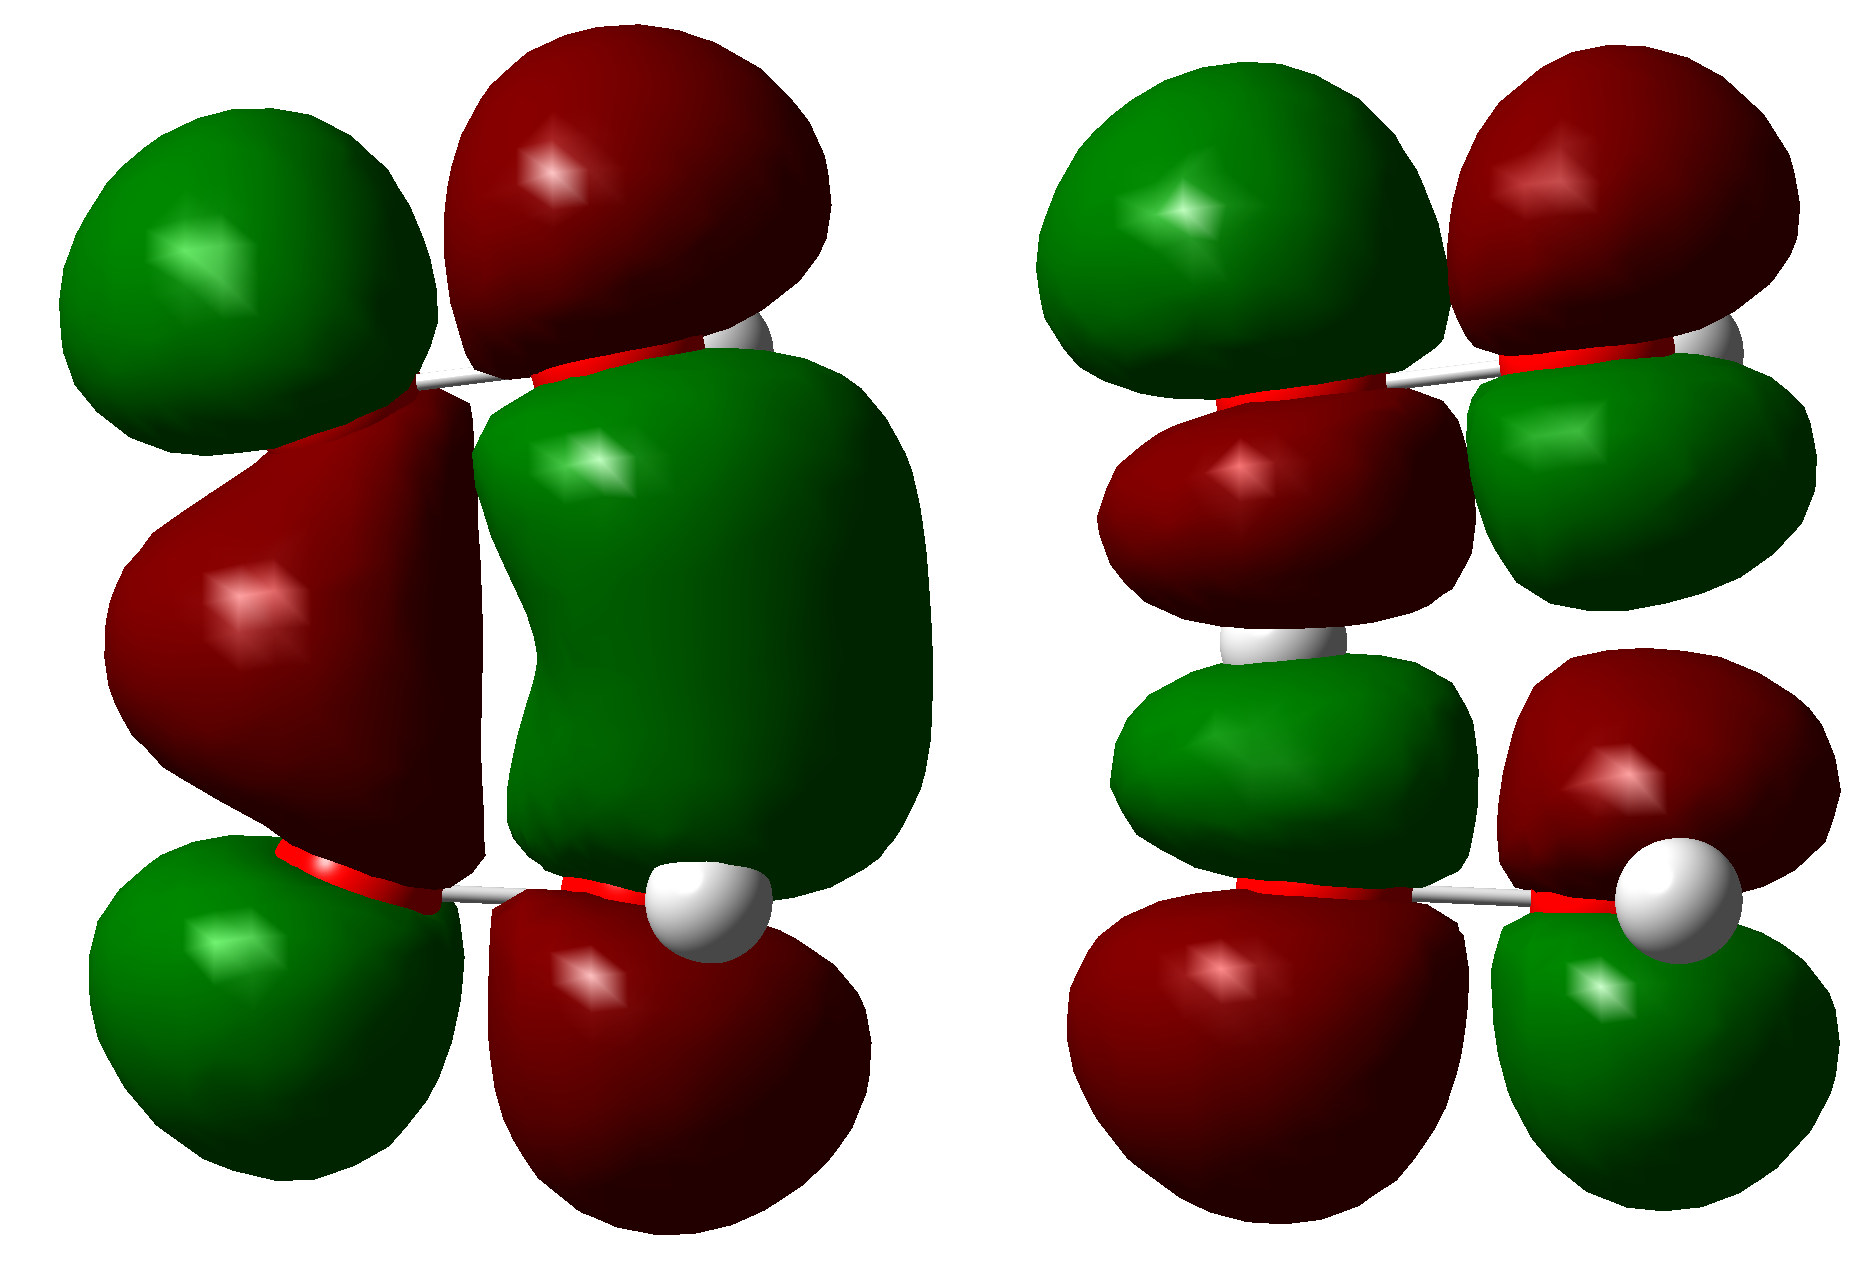
\includegraphics[width=\textwidth]{figures/hoohooh_TS.png}
  \caption[Molecular orbitals of hydrogen peroxide-peroxyl self-exchange
  reaction TS complex, demonstrating a PCET mechanism.]{Molecular orbitals of
  hydrogen peroxide-peroxyl self-exchange reaction TS complex, demonstrating a
  PCET mechanism. Left is the HOMO-1 and right is the SOMO.\@ Together they
  demonstrate a lone pair-lone pair net half bonding interactions, consistent
  with PCET. MOs are shown with an isovalue of 0.02 $e^-/$\AA.}
  \label{fig:hooh-ooh}
\end{figure}

\chapter{Chapter~\protect\ref{ch:bde} Additional Data}\label{ap:bde}

\begin{figure}[H]
\hspace*{-1.8cm}
\begin{minipage}{8cm}
  \centering
  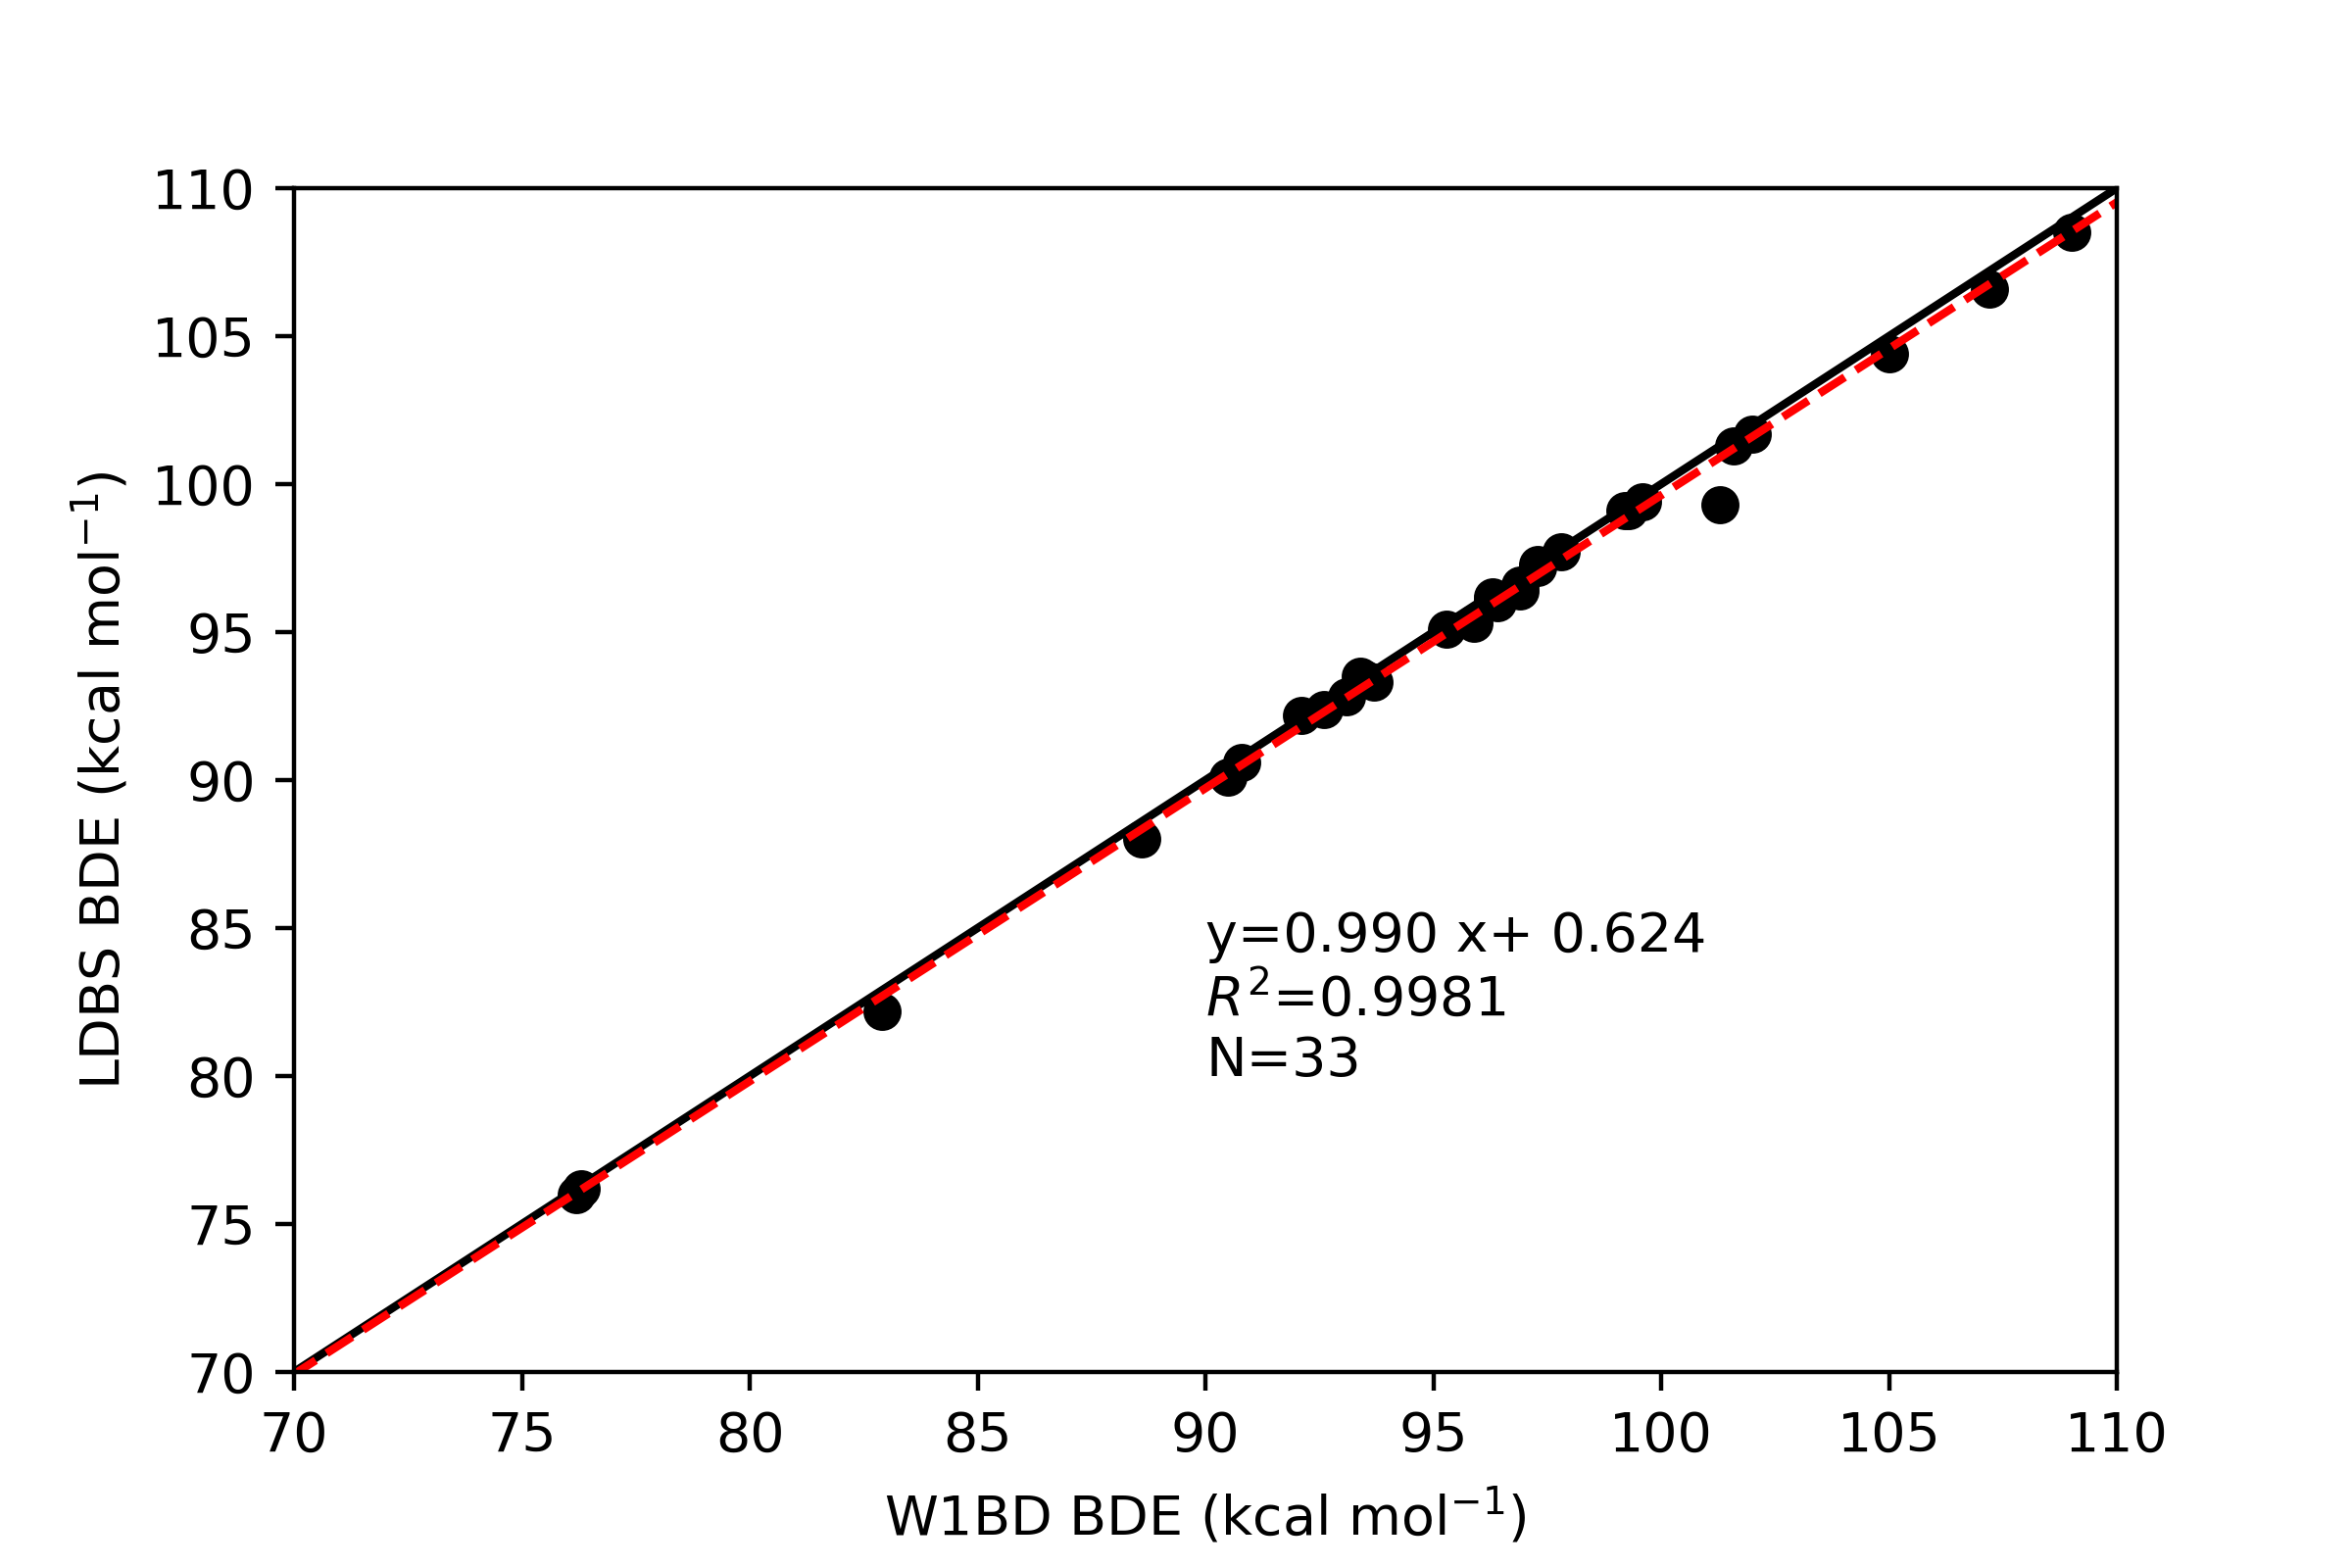
\includegraphics[width=\textwidth]{figures/w1bd-ldbs}
\end{minipage}%
\begin{minipage}{8cm}
  \centering
  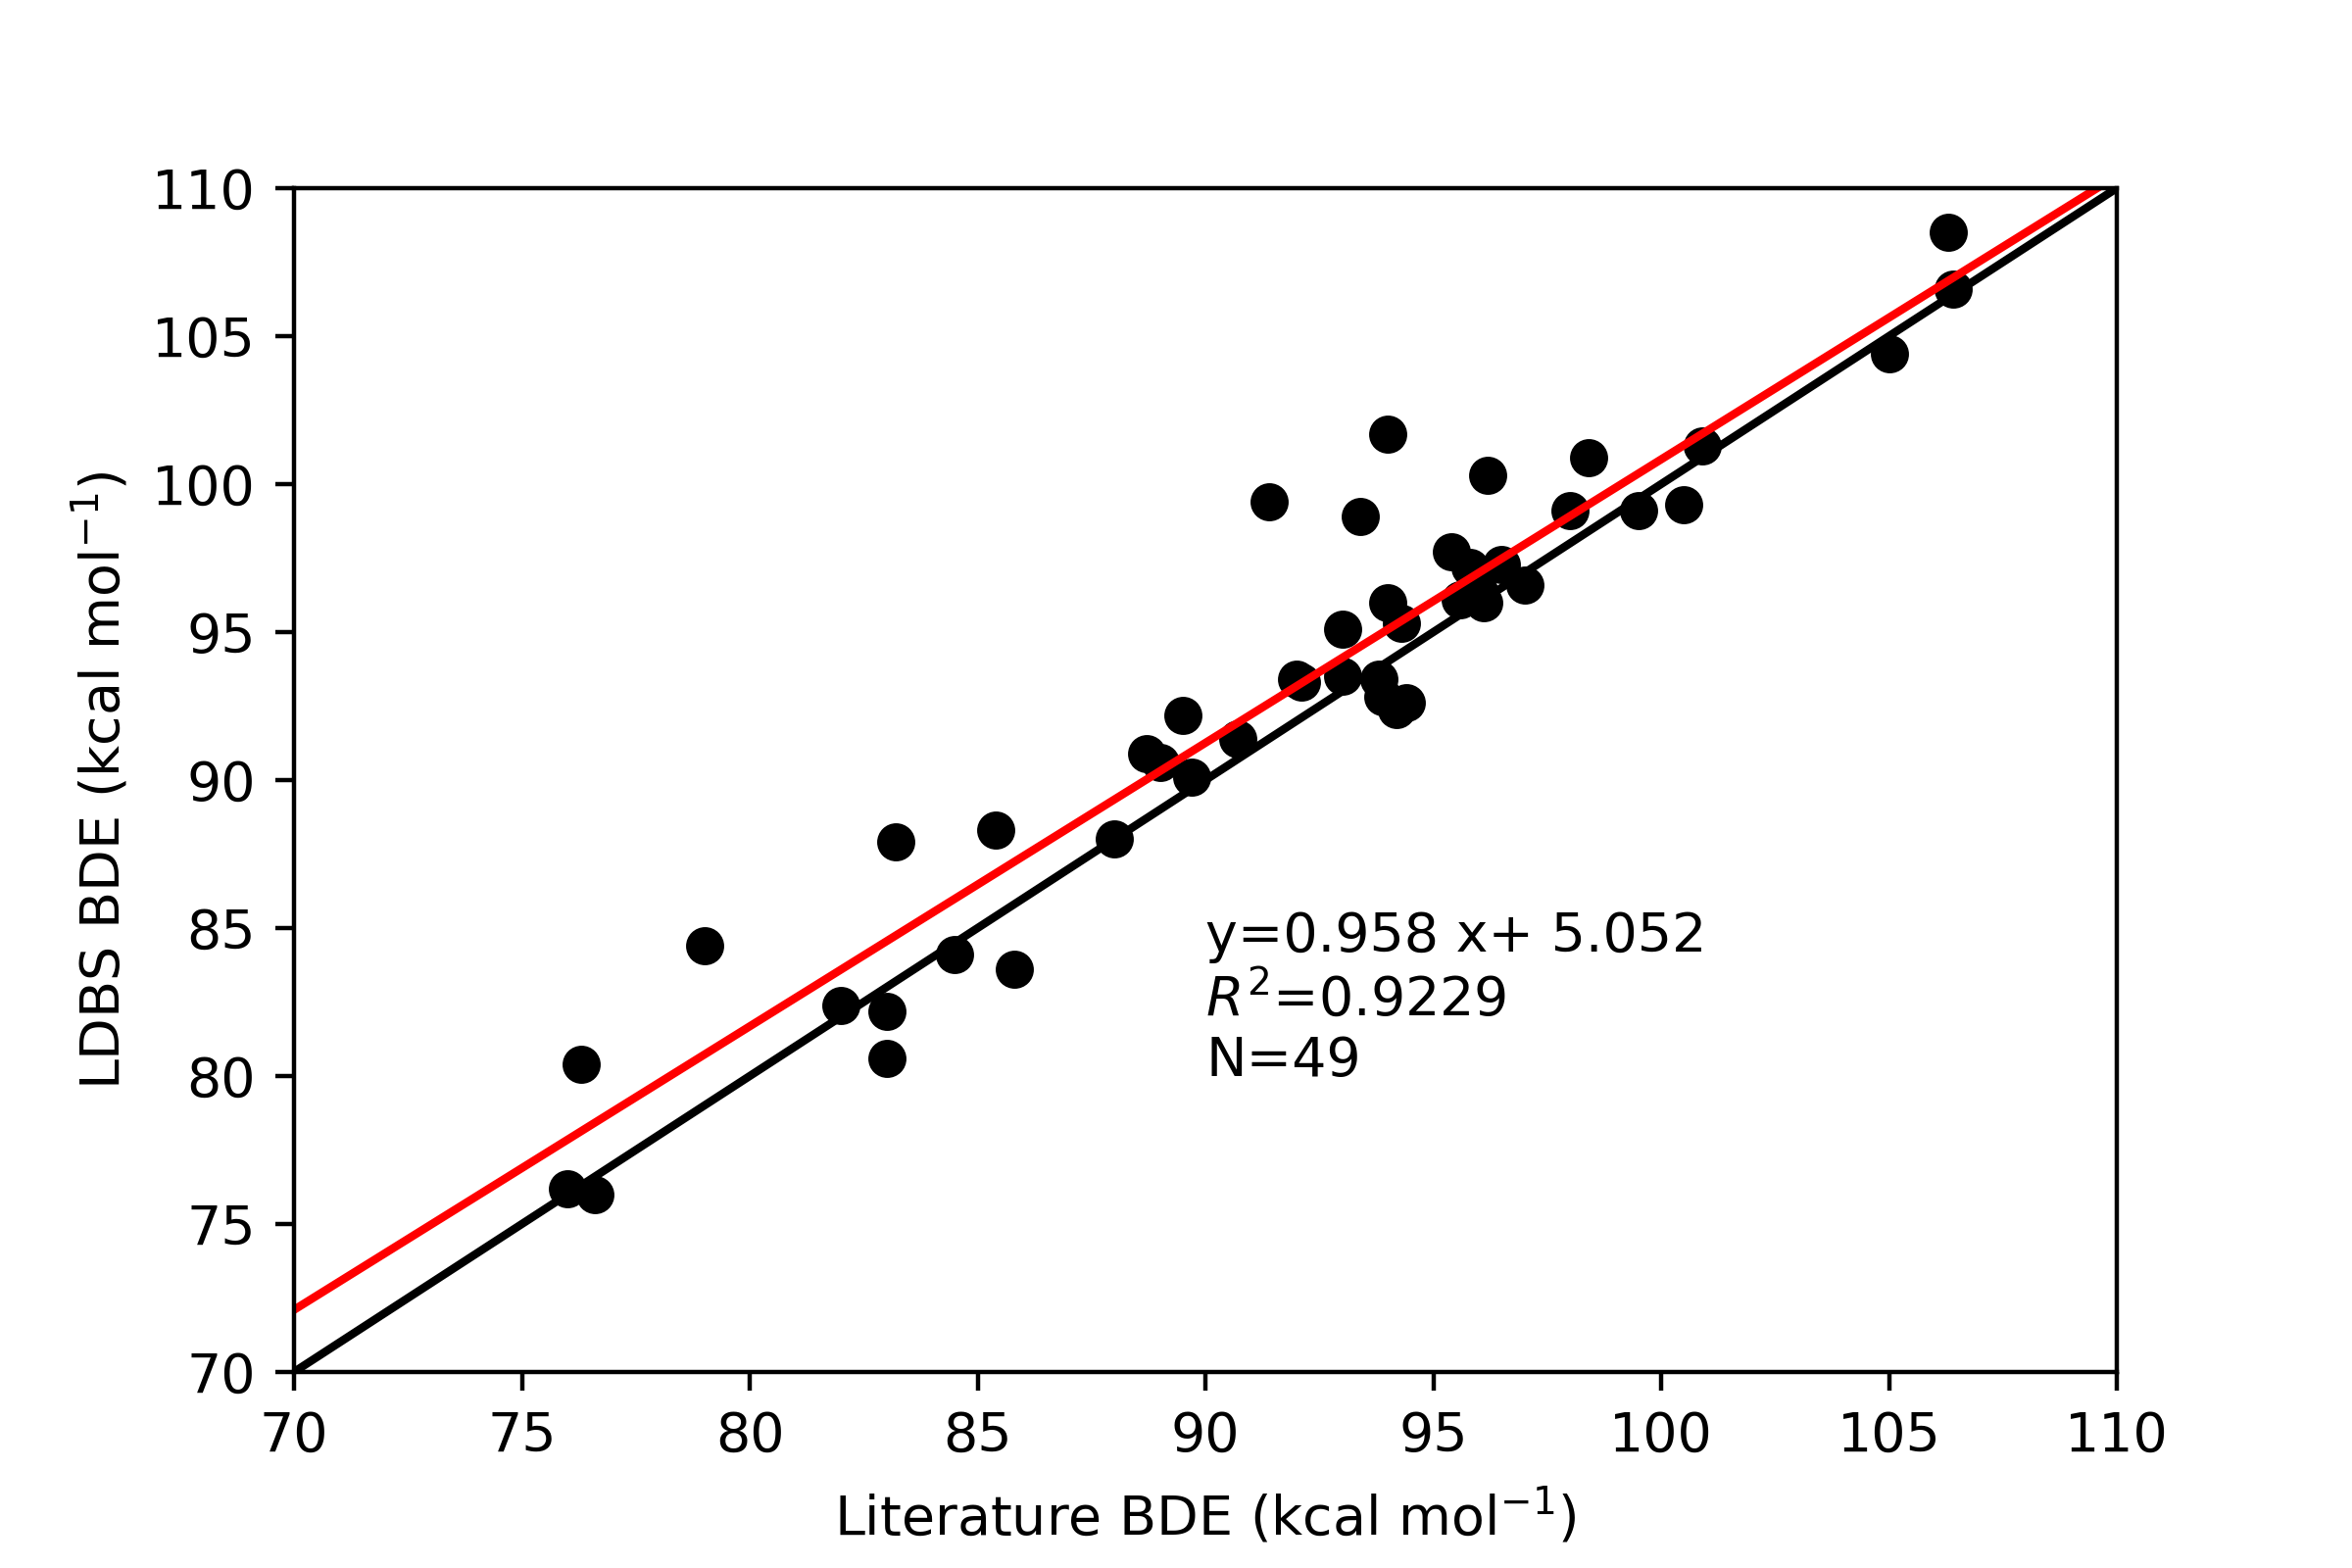
\includegraphics[width=\textwidth]{figures/lit-ldbs}
\end{minipage}

\hspace*{-1.8cm}
\begin{minipage}{8cm}
  \centering
  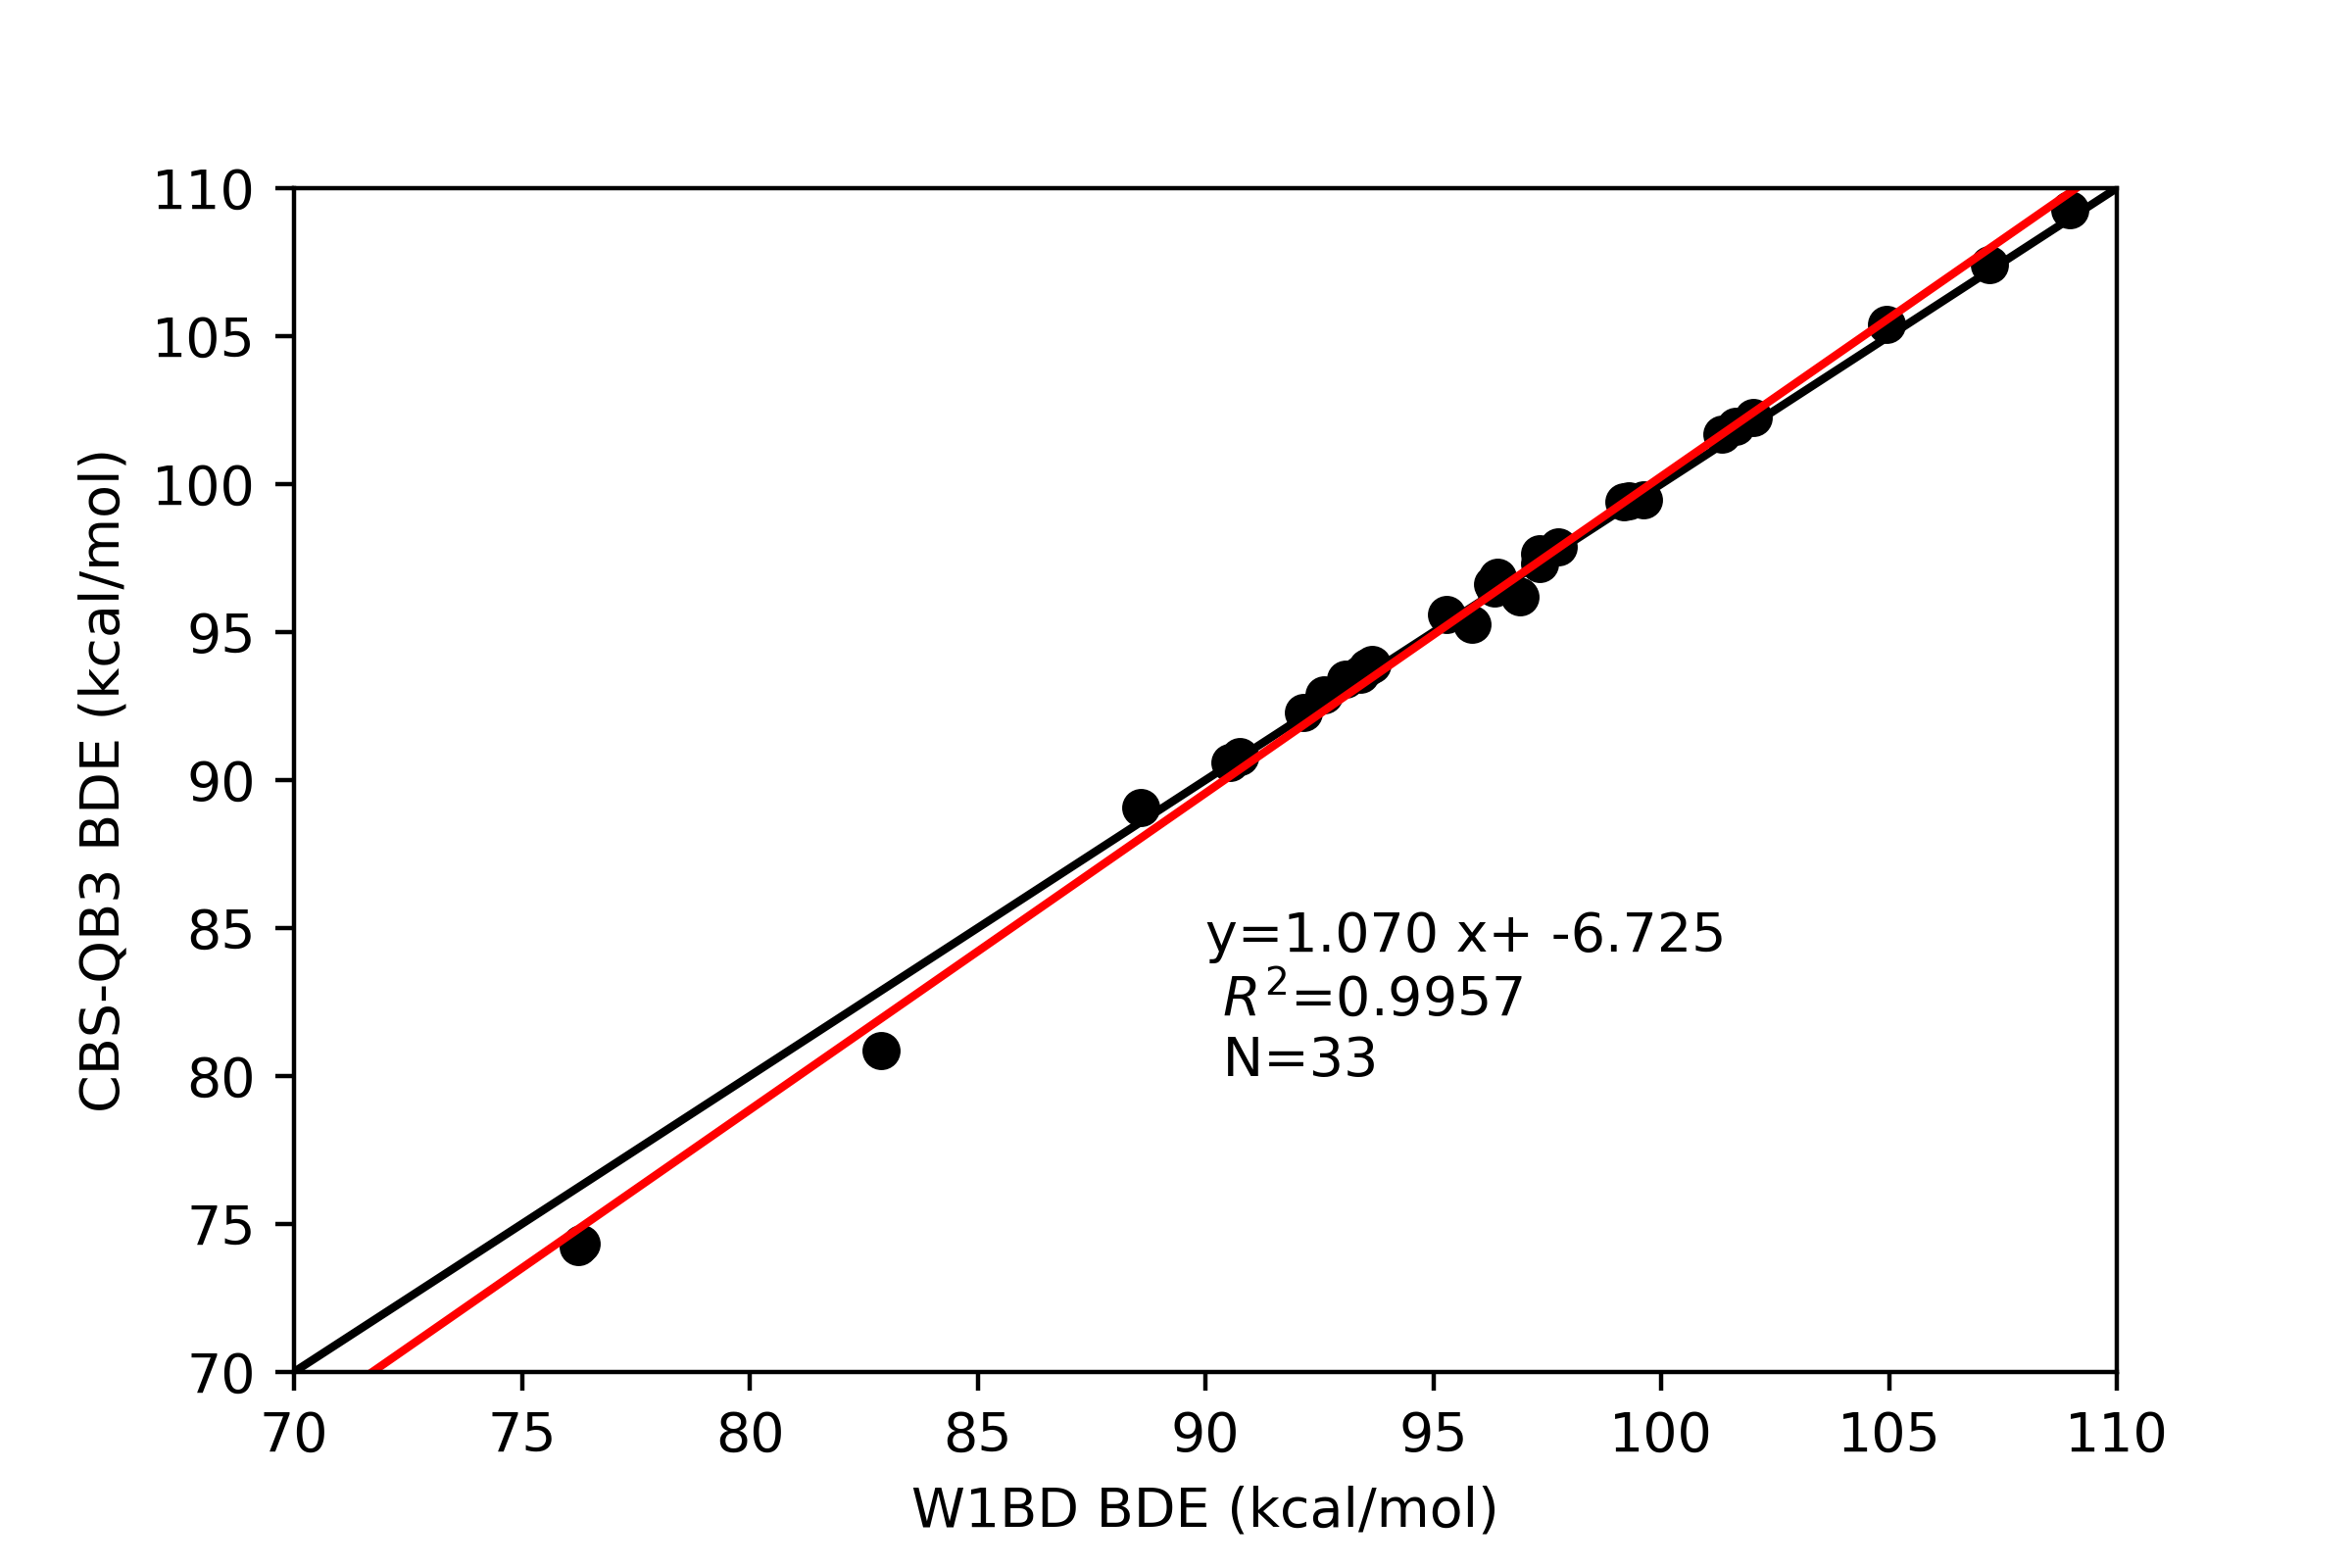
\includegraphics[width=\textwidth]{figures/w1bd-cbsqb3}
\end{minipage}%
\begin{minipage}{8cm}
  \centering
  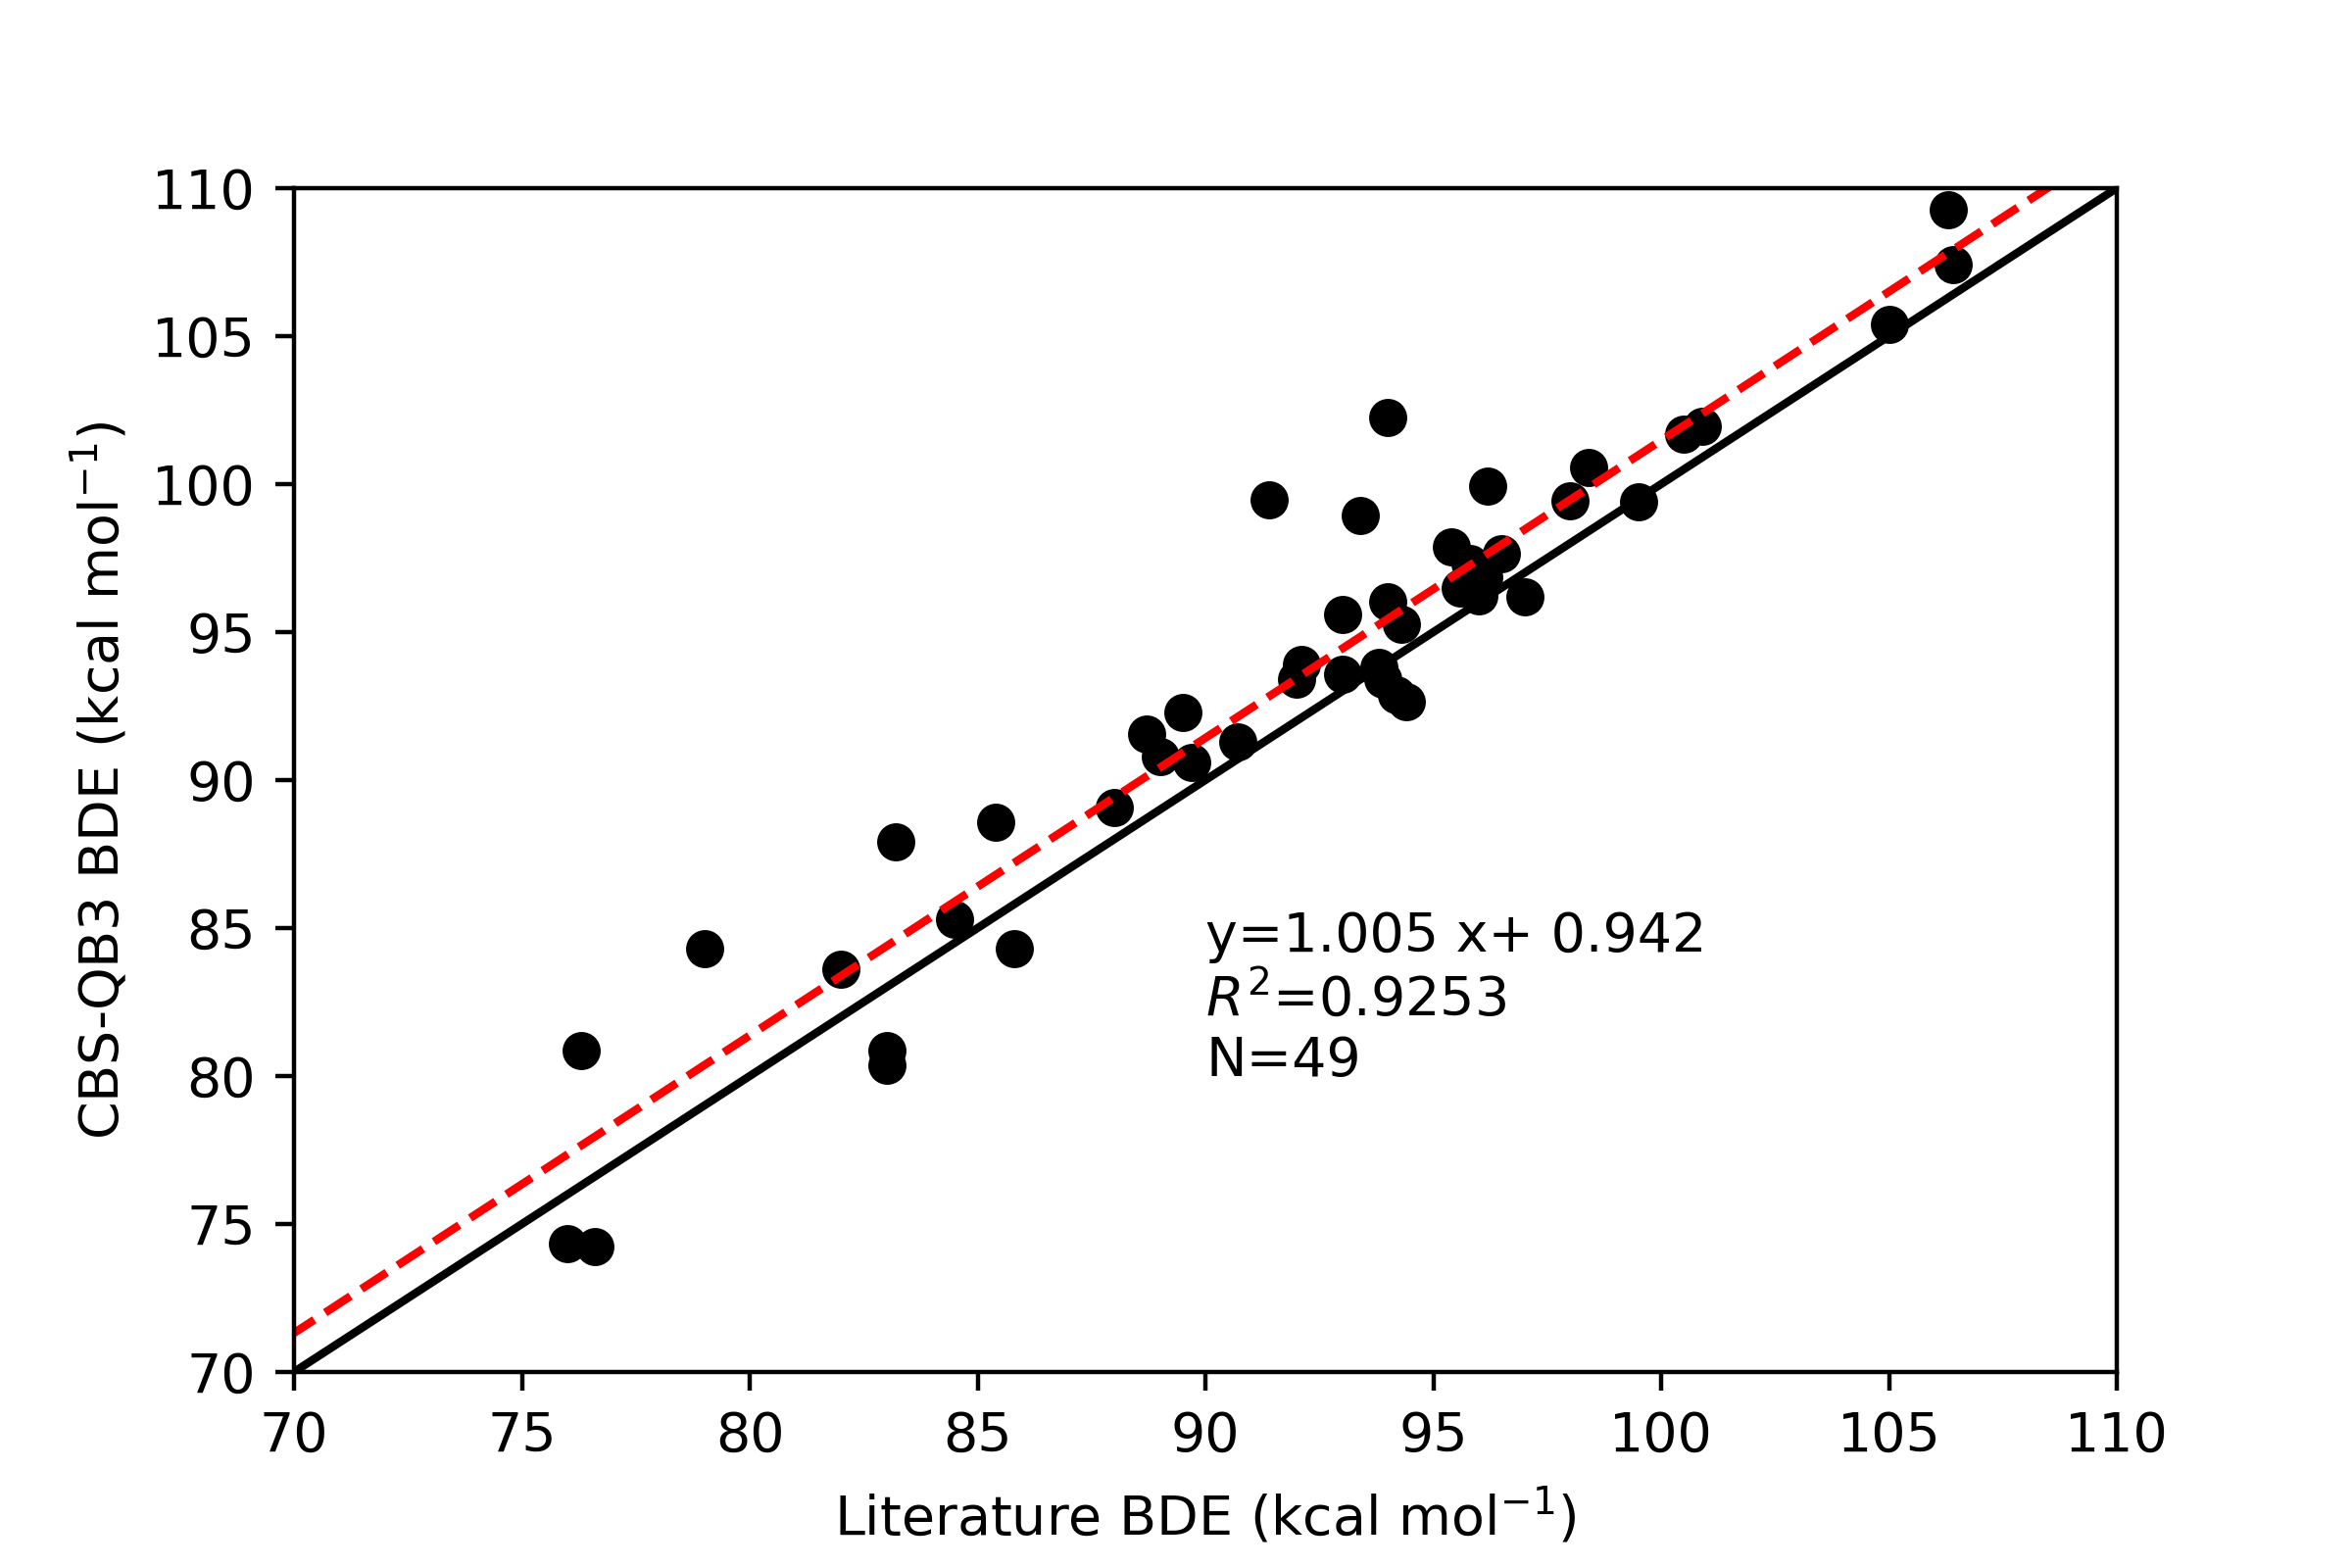
\includegraphics[width=\textwidth]{figures/lit-cbsqb3}
\end{minipage}
\caption{One-to-one plots of composite methods compared to literature and W1BD.}
\end{figure}

\begin{figure}[H]\ContinuedFloat
\hspace*{-1.8cm}
\begin{minipage}{8cm}
  \centering
  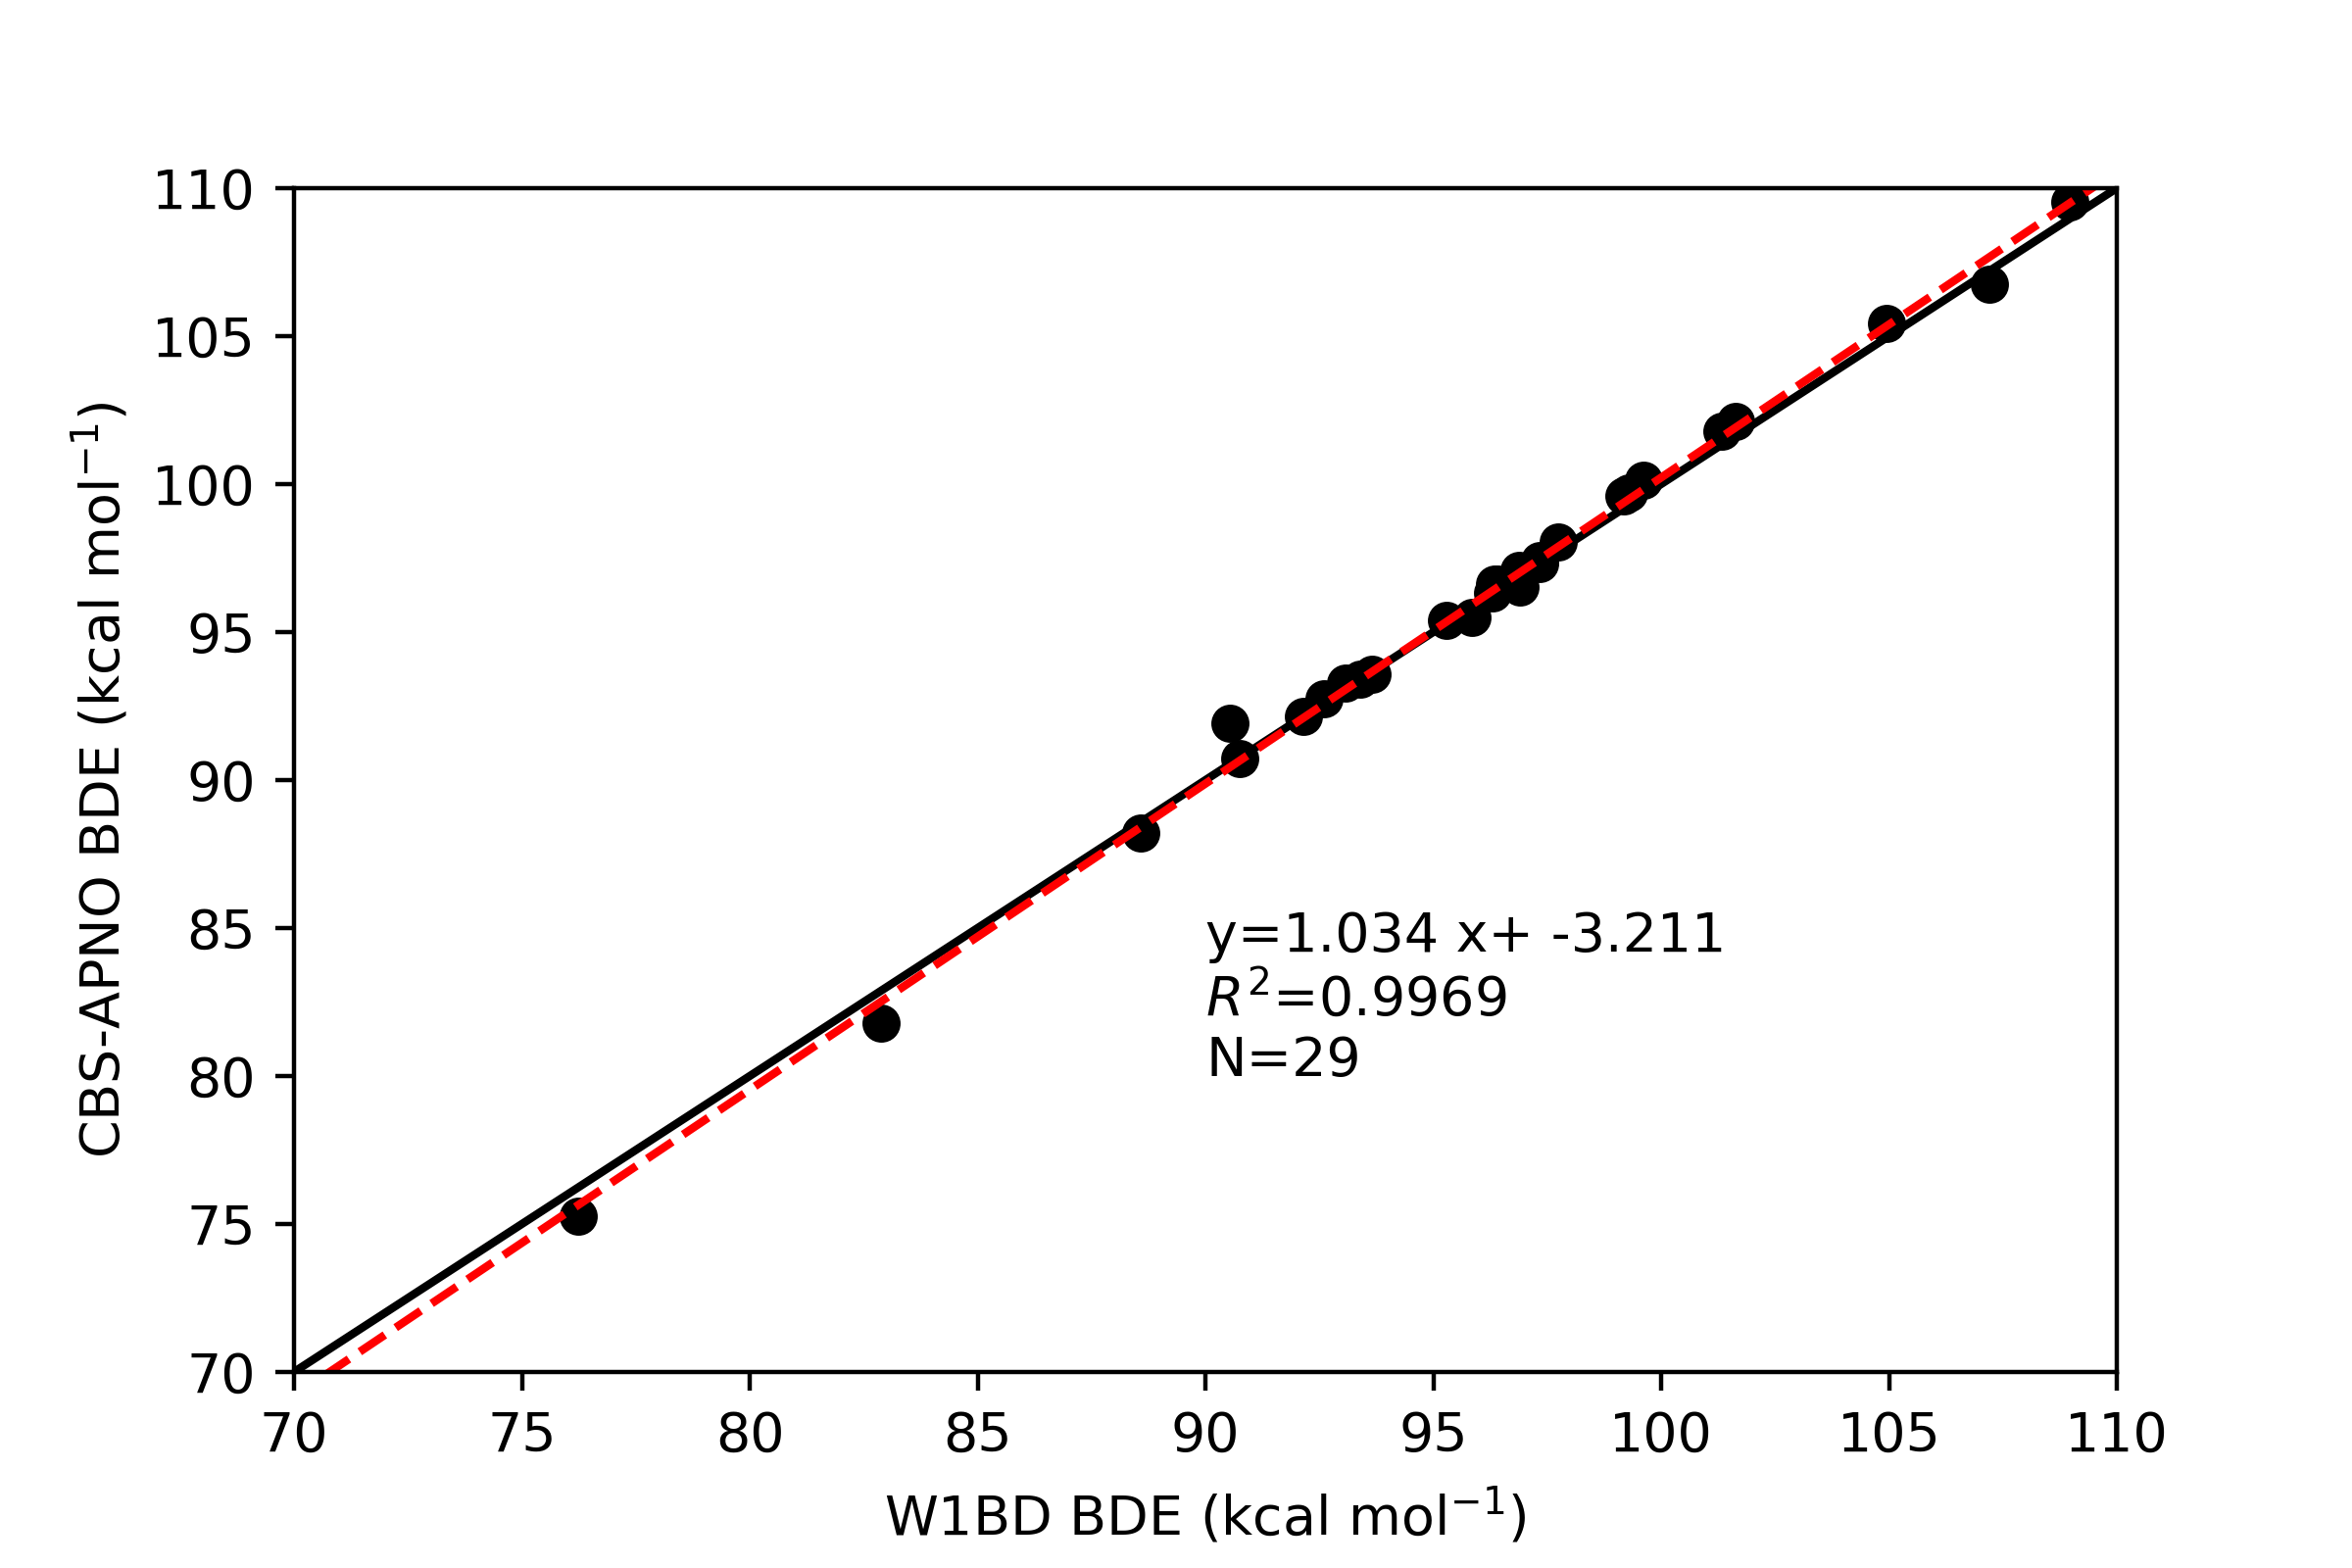
\includegraphics[width=\textwidth]{figures/w1bd-cbsapno}
\end{minipage}%
\begin{minipage}{8cm}
  \centering
  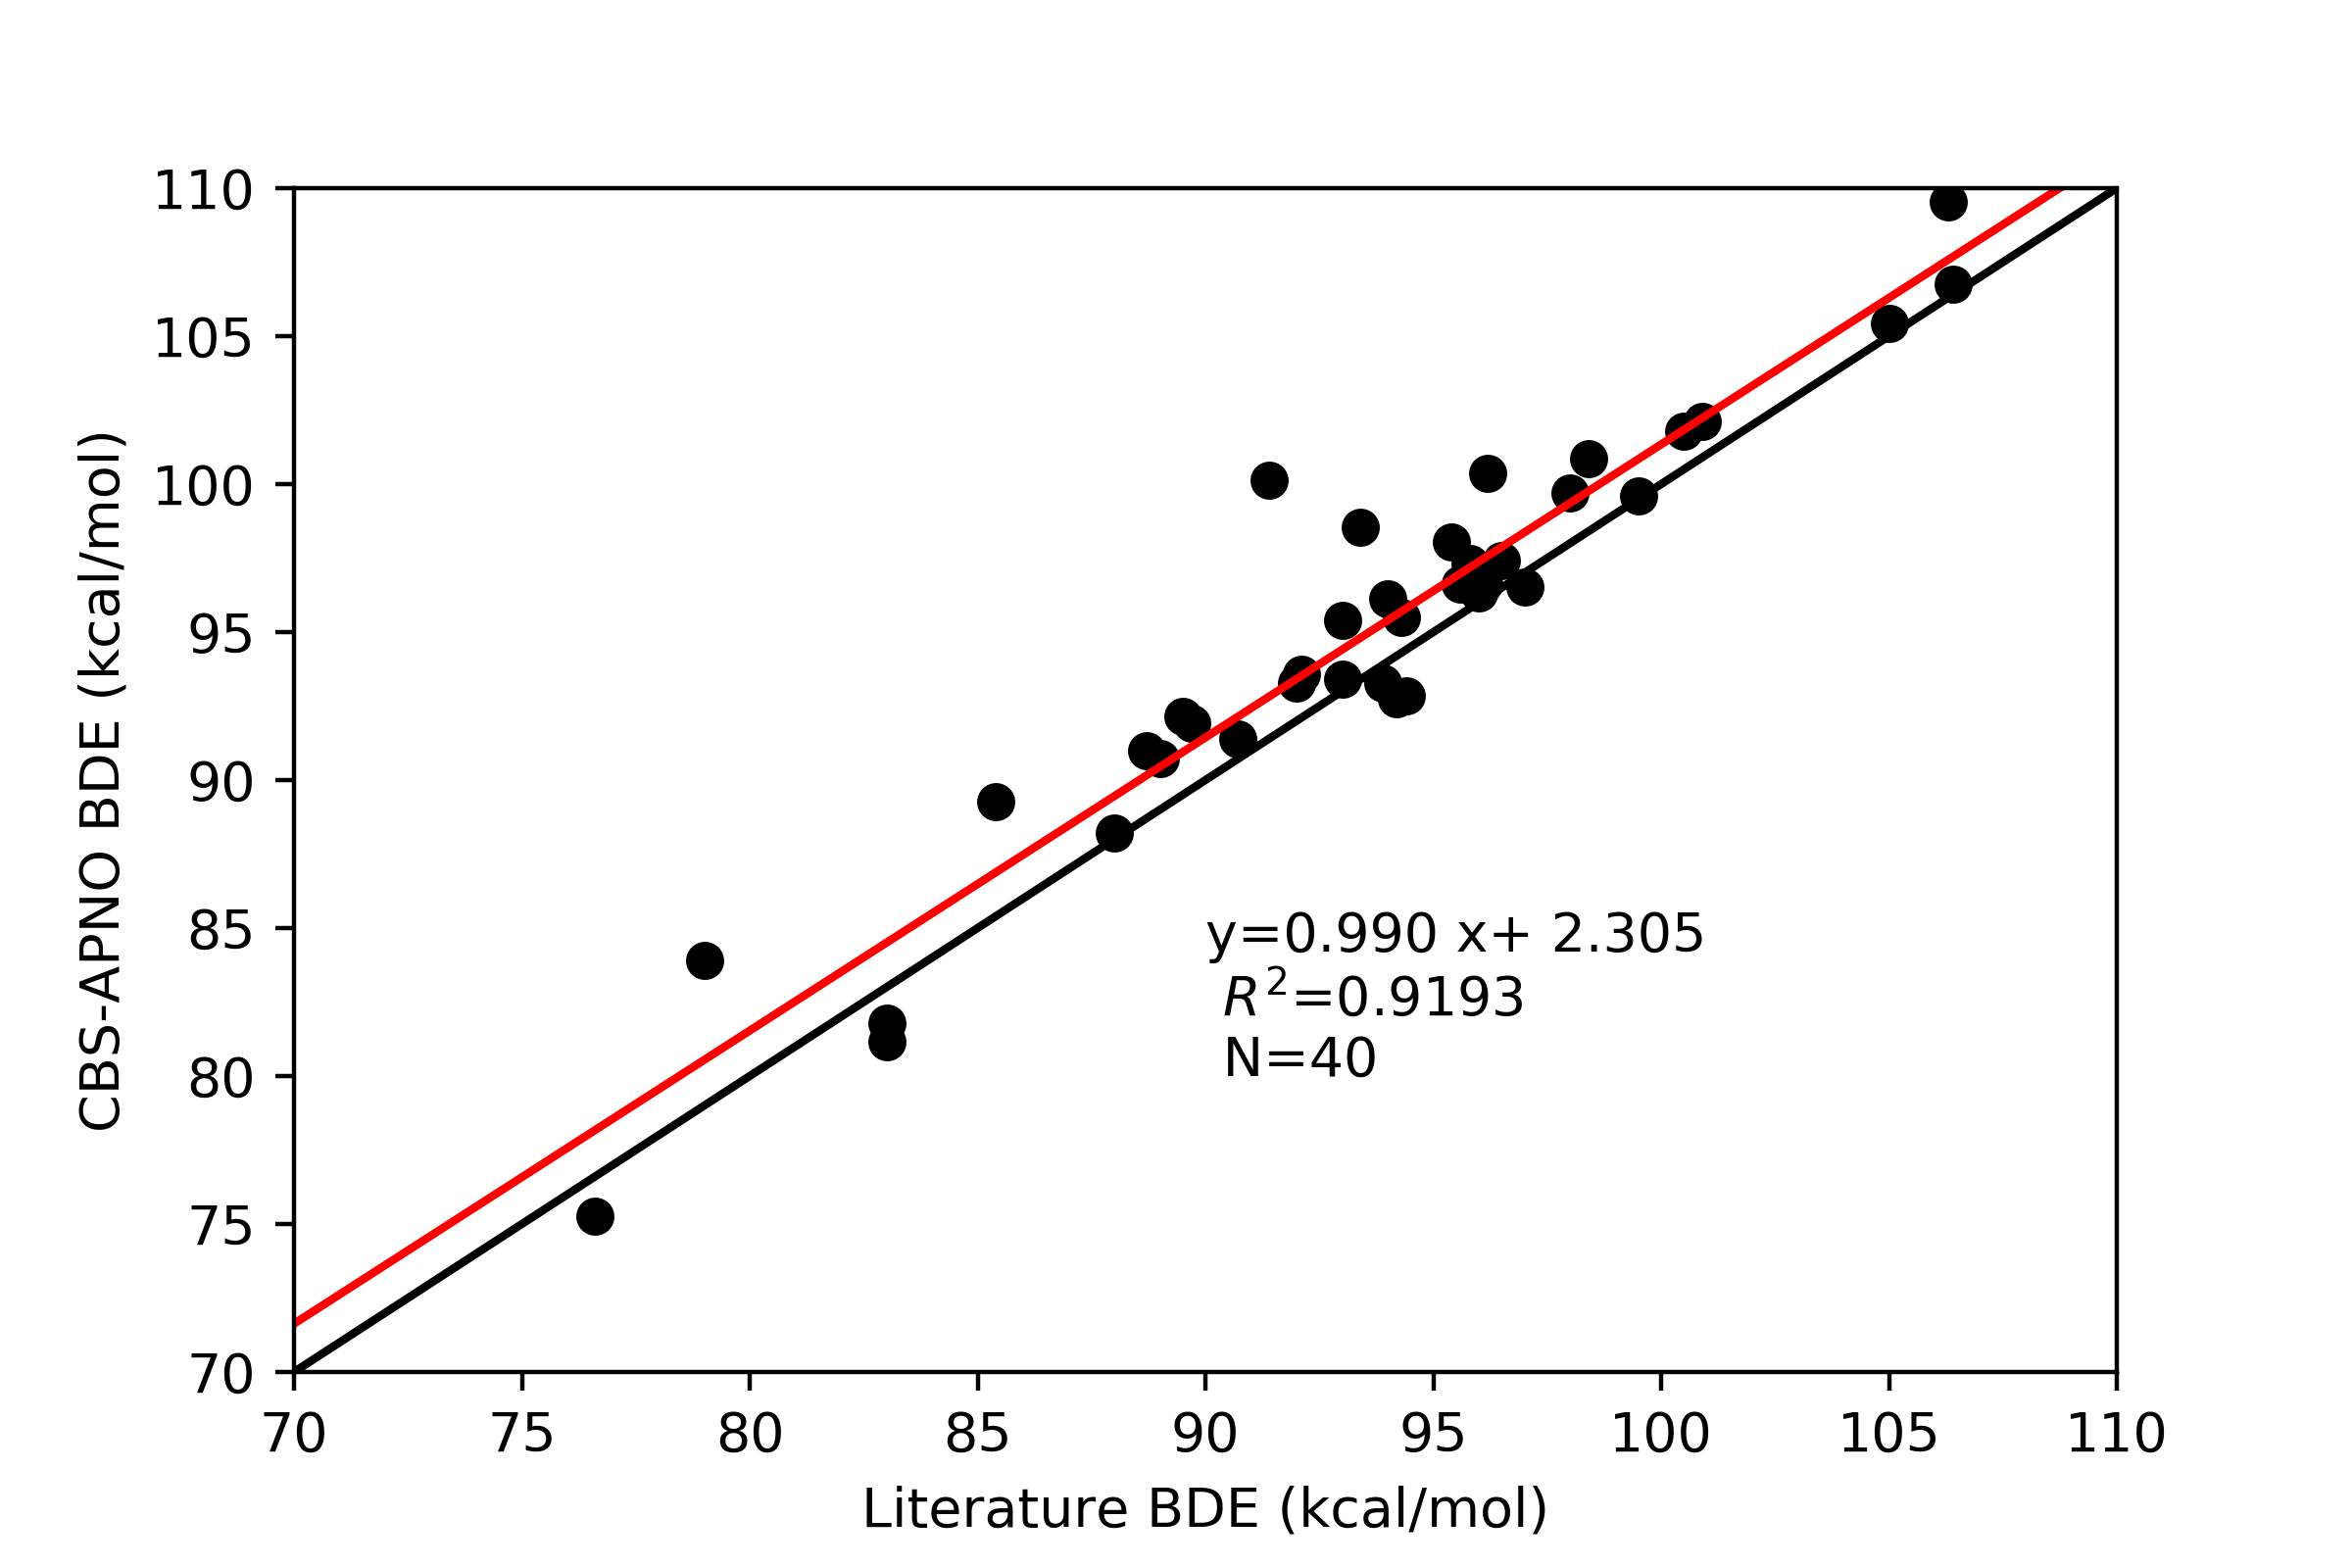
\includegraphics[width=\textwidth]{figures/lit-cbsapno}
\end{minipage}

\hspace*{-1.8cm}
\begin{minipage}{8cm}
  \centering
  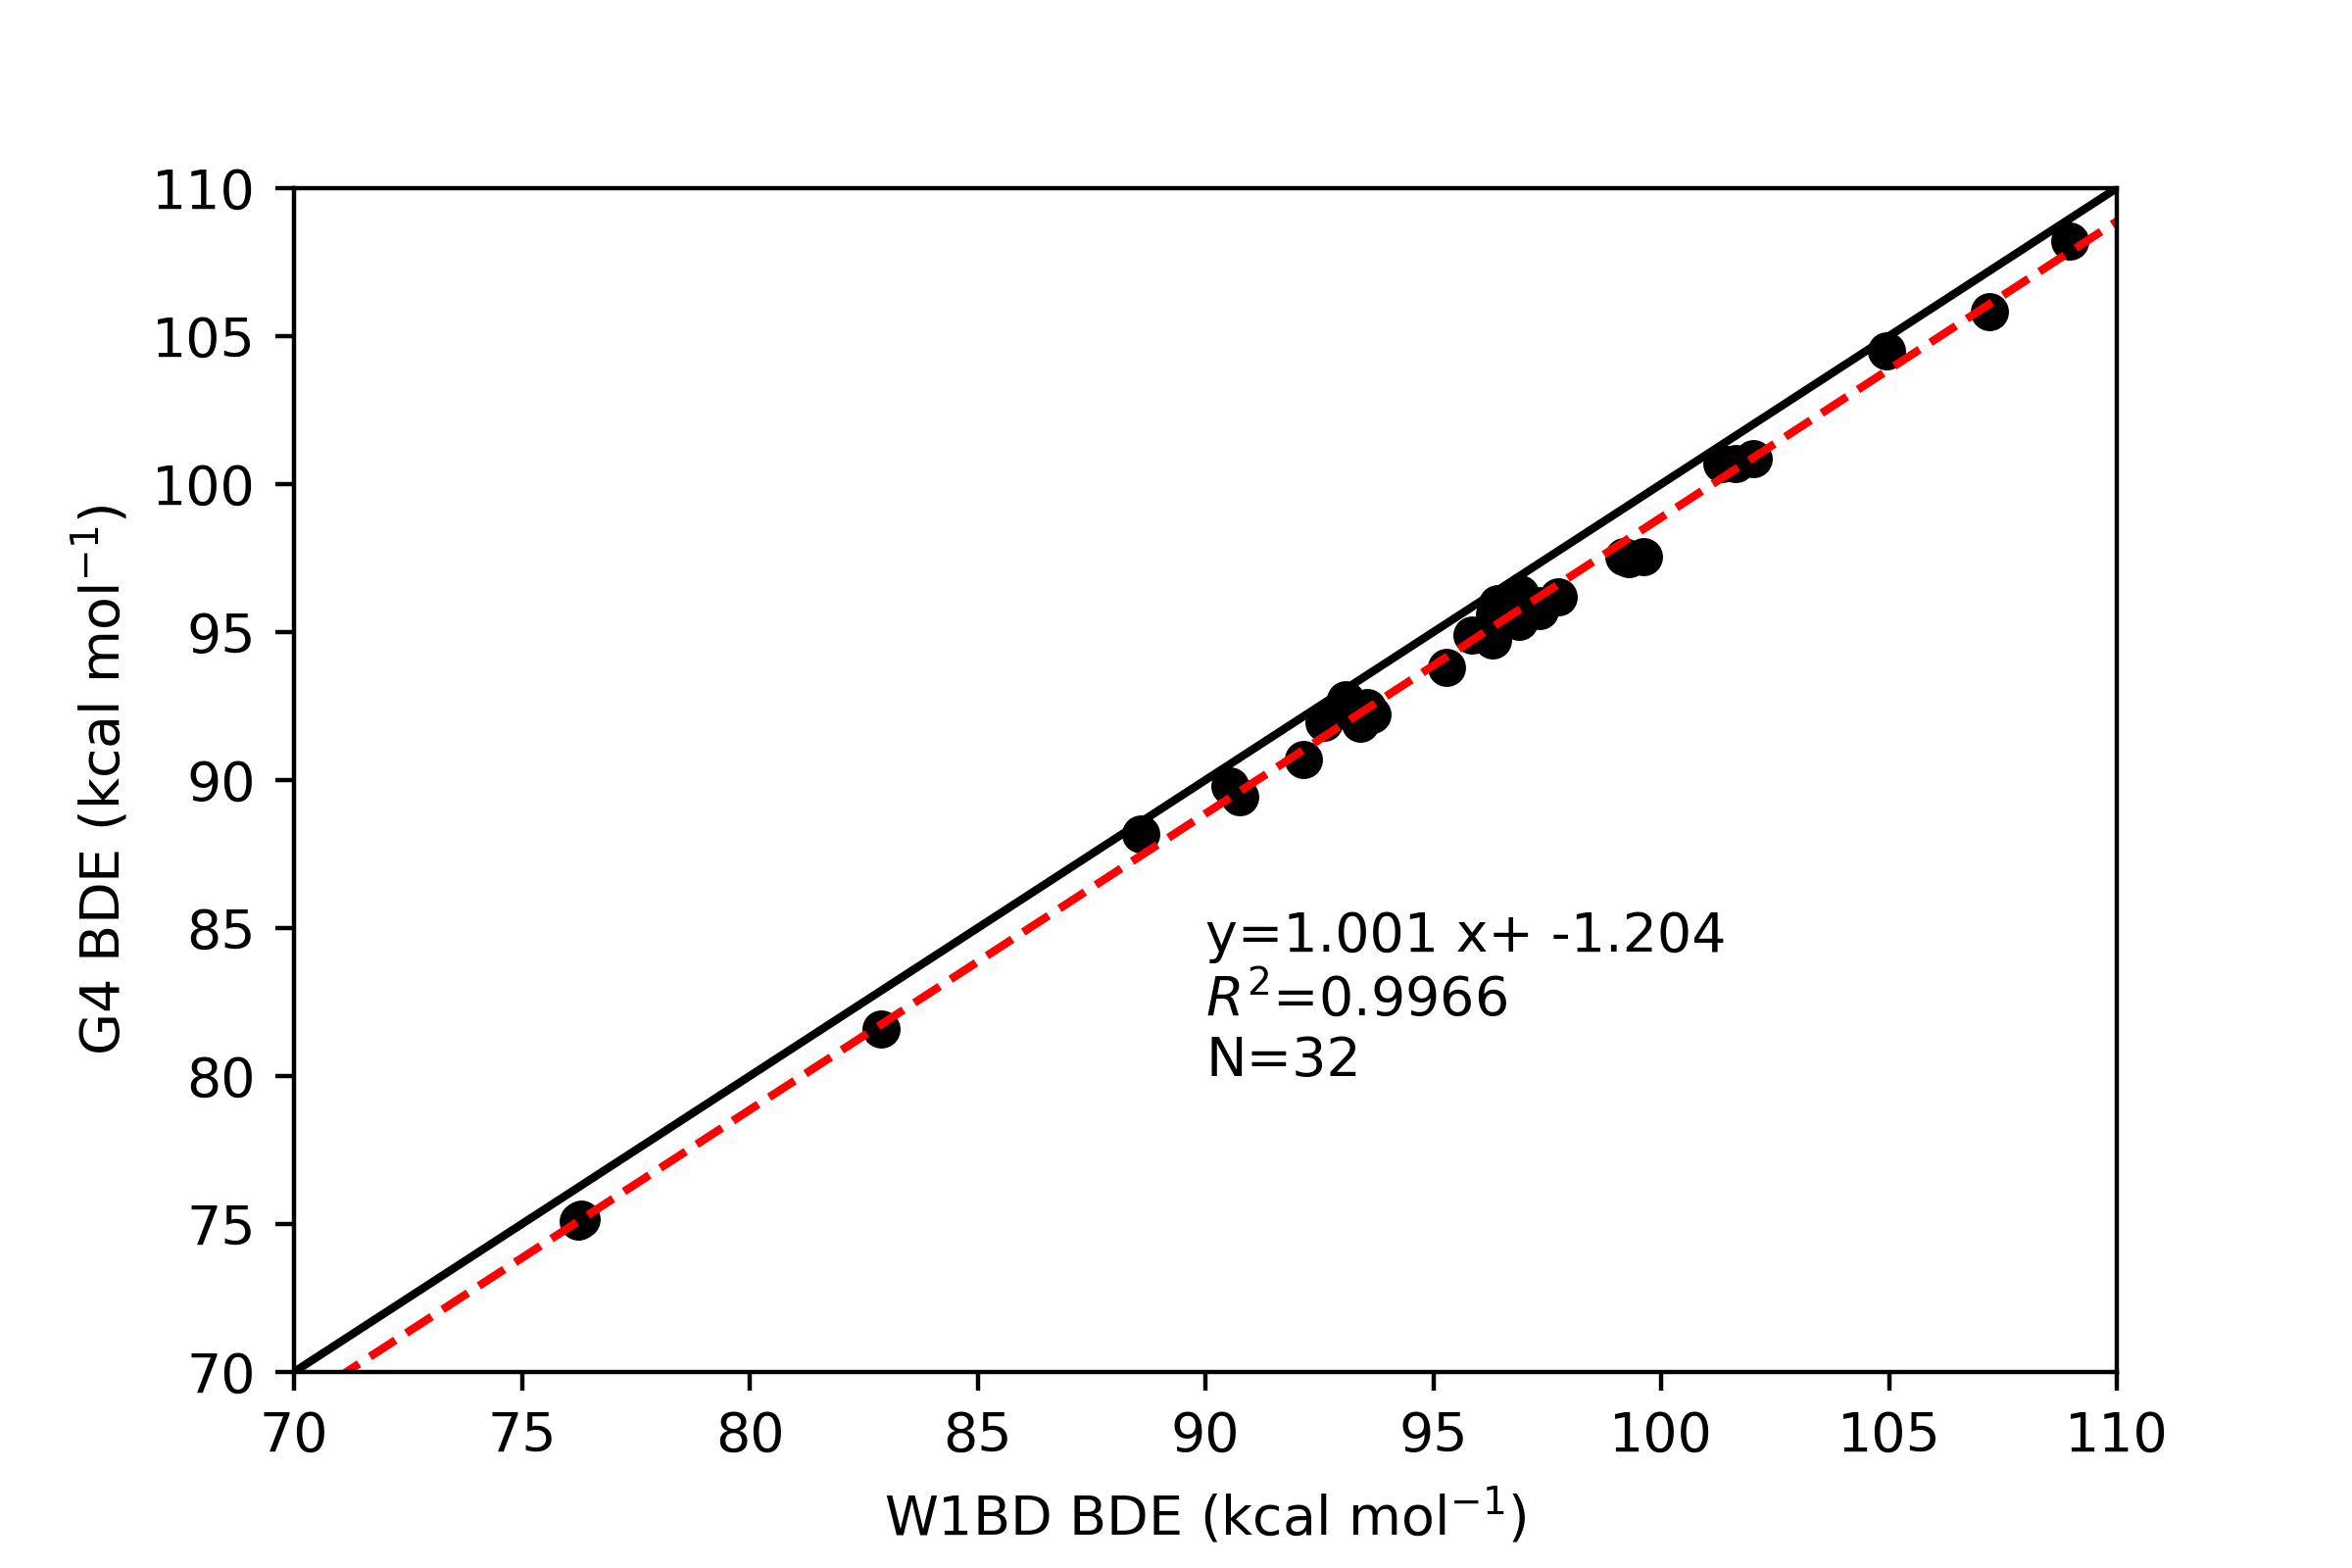
\includegraphics[width=\textwidth]{figures/w1bd-g4}
\end{minipage}%
\begin{minipage}{8cm}
  \centering
  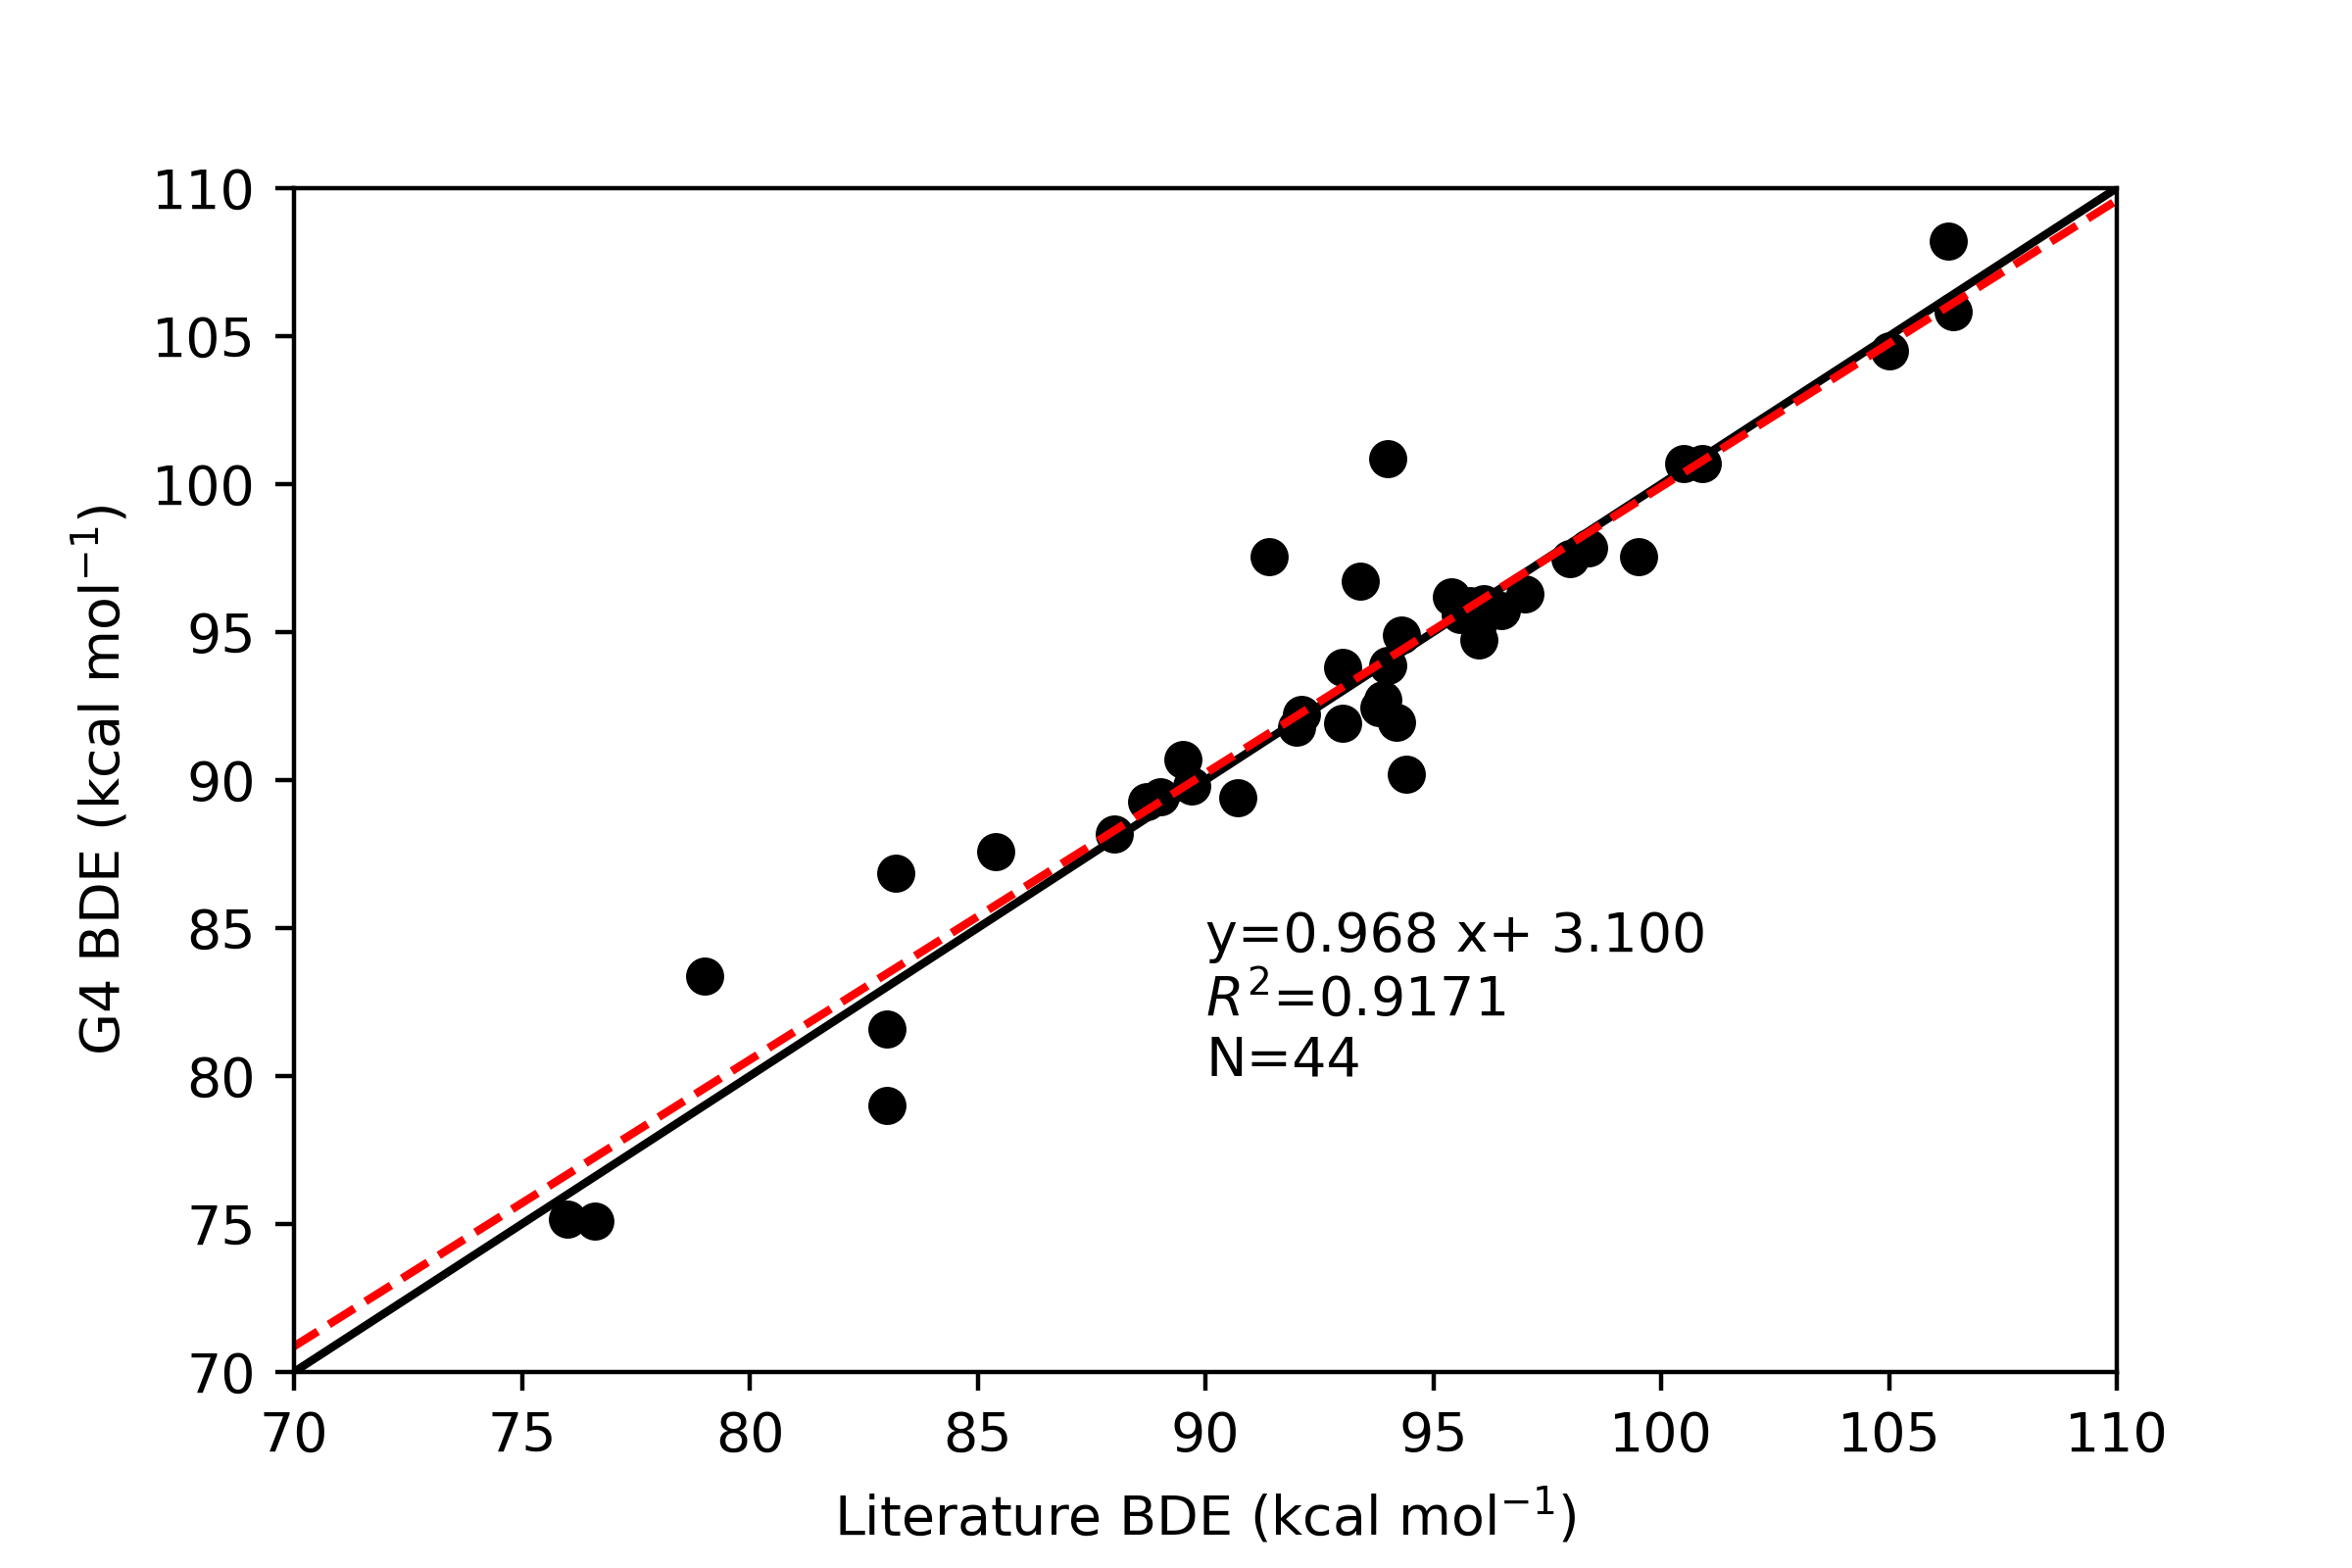
\includegraphics[width=\textwidth]{figures/lit-g4}
\end{minipage}
\caption[]{Continued: One-to-one plots of composite methods compared to
literature and W1BD.}
\end{figure}

\begin{figure}[H]\ContinuedFloat
\hspace*{-1.8cm}
\begin{minipage}{8cm}
  \centering
  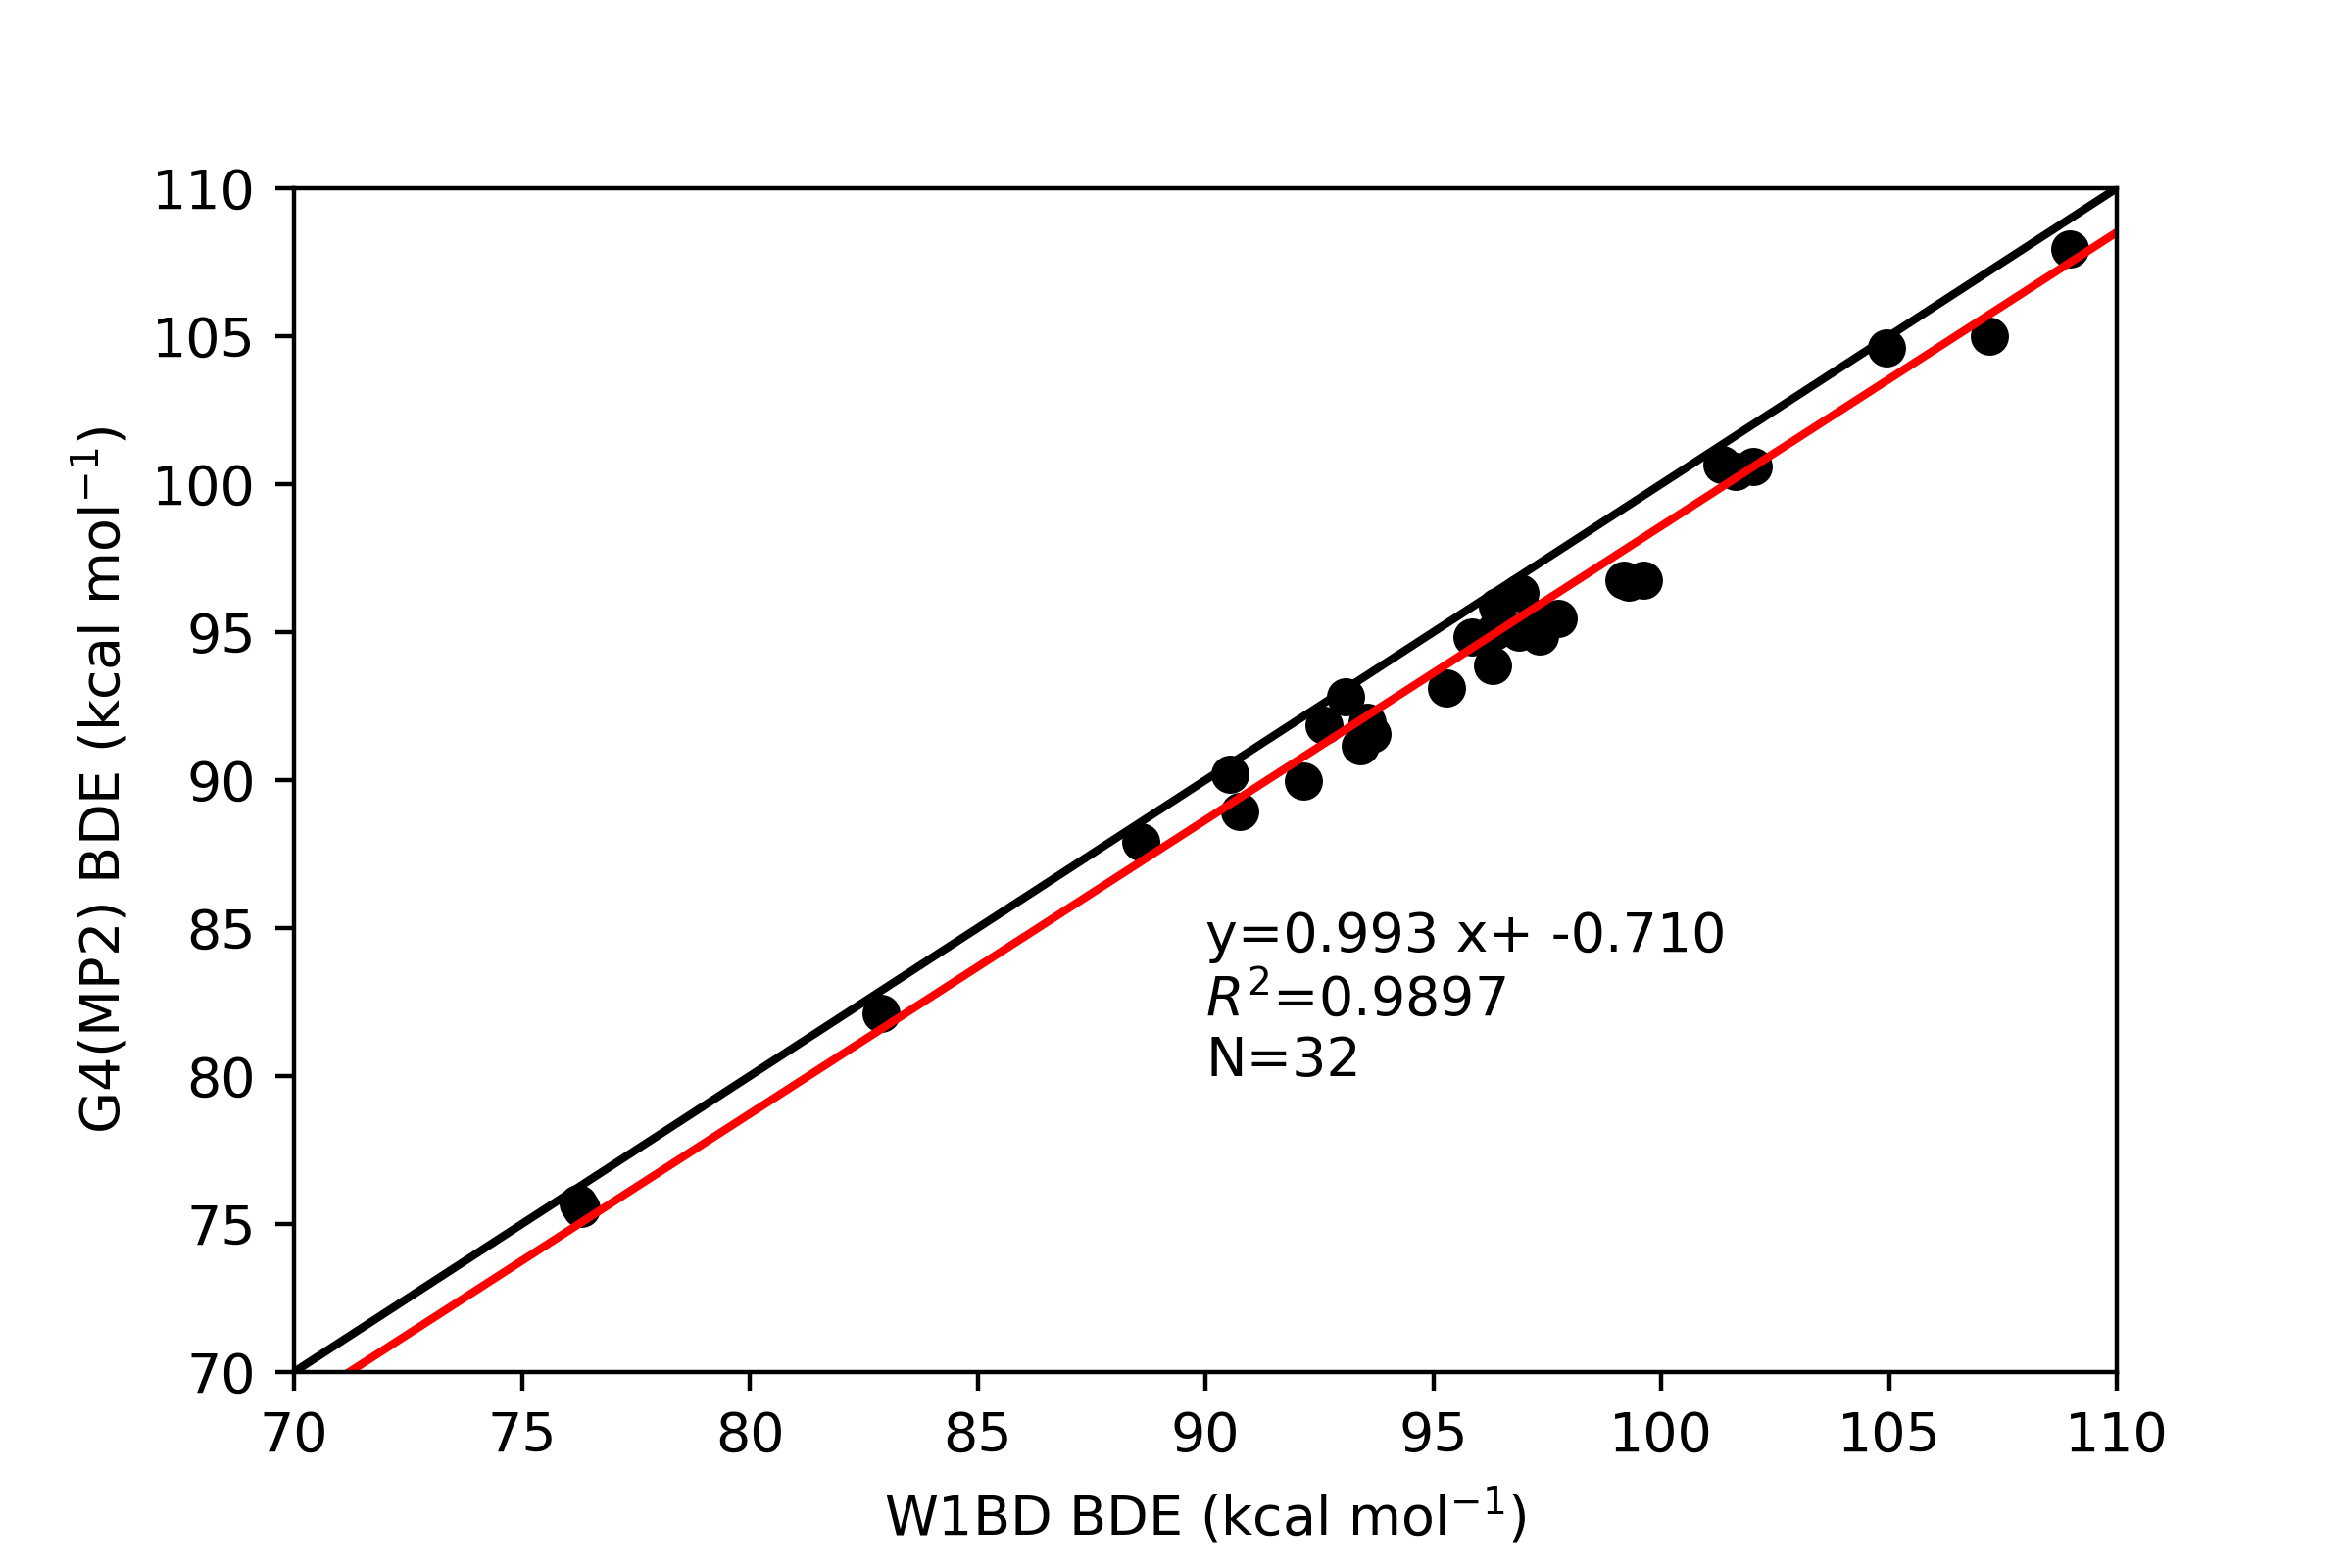
\includegraphics[width=\textwidth]{figures/w1bd-g4mp2}
\end{minipage}%
\begin{minipage}{8cm}
  \centering
  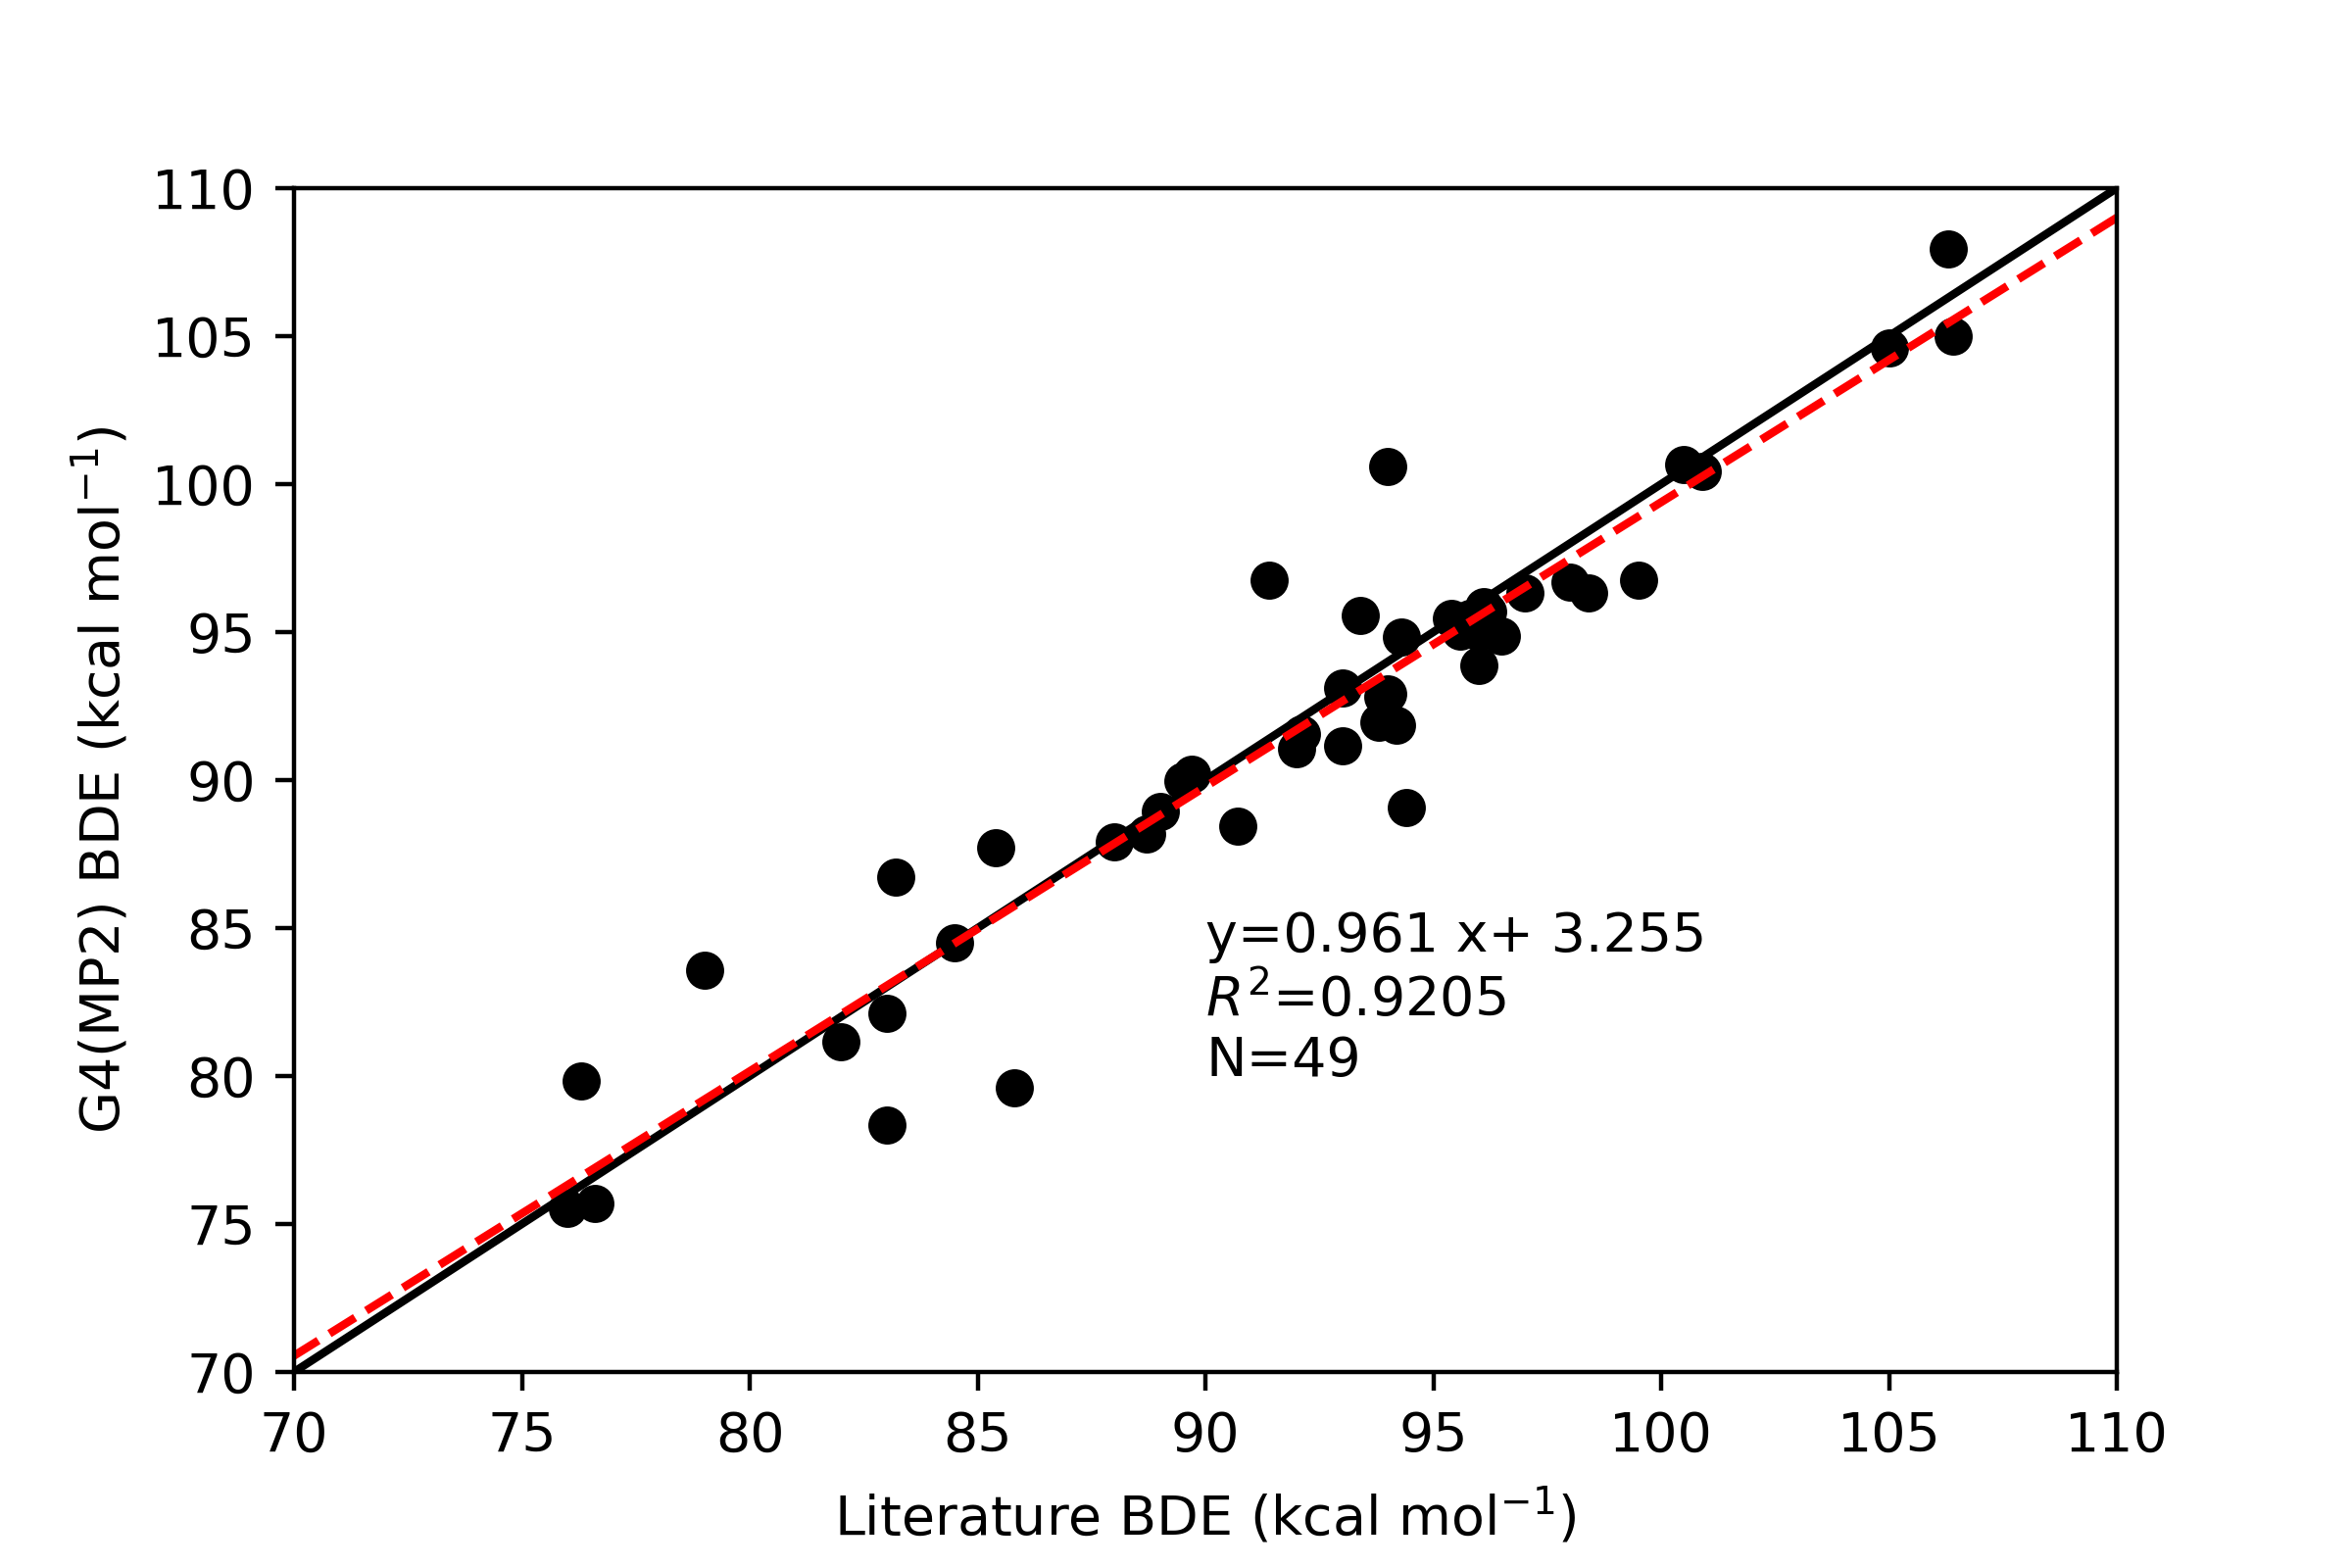
\includegraphics[width=\textwidth]{figures/lit-g4mp2}
\end{minipage}
\caption[]{Continued: One-to-one plots of composite methods compared to
literature and W1BD.}
\end{figure}

\begin{longtable}{m{3.1cm} | c c c}
\caption[Summary of experimental rate constants and literature bond dissociation enthalpies (BDEs).]{Summary of experimental rate constants and literature\cite{Luo2002} bond dissociation enthalpies (BDEs).} \label{tab:expt-bde} \\
\centering
 Molecule                       & $k_H$ \Ms          & Normalized $k_H$ \Ms & BDE \kcalmol \\
\toprule
 1,4-cyclohexadiene             & $ 6.60 \times 10^7$ & $1.65 \times 10^7 $ &        76 \\
 1,4-diazabicyclo-[2.2.2]octane  & $ 9.60 \times 10^6$ & $8.00 \times 10^5 $ &      93.4 \\
 2,2-dimethylbutane             & $ 9.50 \times 10^4$ & $4.75 \times 10^4 $ &        98 \\
 2,3-dimethylbutane             & $ 5.60 \times 10^5$ & $2.80 \times 10^5 $ &      95.4 \\
 9,10-dihydroanthracene         & $ 5.04 \times 10^7$ & $1.26 \times 10^7 $ &      76.3 \\
 Acetone                        & $ < 1 \times 10^4 $ & $2 \times 10^3    $ &        96 \\
 Acetonitrile                   & $ < 1 \times 10^4 $ & $2 \times 10^3    $ &        97 \\
 Adamantane (2$^\circ$)                & $ 6.90 \times 10^6$ & $5.75 \times 10^5 $ &      98.4 \\
 Adamantane (3$^\circ$)                & $ 6.90 \times 10^6$ & $1.73 \times 10^6 $ &      96.2 \\
 Benzaldehyde                   & $ 1.20 \times 10^7$ & $1.20 \times 10^7 $ &      88.7 \\
 Benzyl alcohol                 & $ 2.97 \times 10^6$ & $1.49 \times 10^6 $ &        79 \\
 Cumene                         & $ 5.60 \times 10^5$ & $5.60 \times 10^5 $ &      83.2 \\
 Cycloheptane                   & $ 2.20 \times 10^6$ & $1.57 \times 10^5 $ &        94 \\
 Cyclohexane                    & $ 1.10 \times 10^6$ & $9.17 \times 10^4 $ &      99.5 \\
 Cyclooctane                    & $ 2.98 \times 10^6$ & $1.86 \times 10^5 $ &      94.4 \\
 Cyclopentane                   & $ 9.54 \times 10^6$ & $9.54 \times 10^5 $ &      95.6 \\
 Dibenzyl ether                 & $ 5.60 \times 10^6$ & $1.40 \times 10^6 $ &      85.8 \\
 Diethyl ether                  & $ 2.60 \times 10^6$ & $6.50 \times 10^5 $ &        93 \\
 Dimethyl sulfoxide              & $ 1.80 \times 10^4$ & $6.00 \times 10^3 $ &        94 \\
 Dioxane                        & $ 8.20 \times 10^5$ & $1.03 \times 10^5 $ &      96.5 \\
 Diphenylmethane                & $ 8.71 \times 10^5$ & $4.36 \times 10^5 $ &      84.5 \\
 Ethylbenzene                   & $ 7.90 \times 10^5$ & $3.95 \times 10^5 $ &      85.4 \\
 Hexamethyl-phorsphoramide       & $ 1.87 \times 10^7$ & $1.04 \times 10^6 $ &           \\
 Morpholine                     & $ 5.00 \times 10^7$ & $1.25 \times 10^7 $ &        92 \\
 Piperazine                     & $ 2.4 \times 10^8 $ &                &        93 \\
 Piperidine                     & $ 1.2 \times 10^8 $ &                &      89.5 \\
 Pyrrolidine                    & $ 1.1 \times 10^8 $ &                &        89 \\
 Tetrahydro-2H-pyran            & $ 1.4 \times 10^6 $ &                &        96 \\
 Tetrahydrofuran                & $ 5.8 \times 10^6 $ &                &      92.1 \\
 Toluene                        & $ 1.85 \times 10^5$ & $6.17 \times 10^4 $ &      89.7 \\
 Triethylamine                  & $ 2.10 \times 10^8$ & $3.5 \times 10^7  $ &      90.7 \\
 Triphenylmethane               & $ 3.04 \times 10^5$ & $3.04 \times 10^5 $ &        81 \\
\end{longtable}


\begin{figure}[H]
\hspace*{-1.8cm}
\begin{minipage}{8cm}
  \centering
  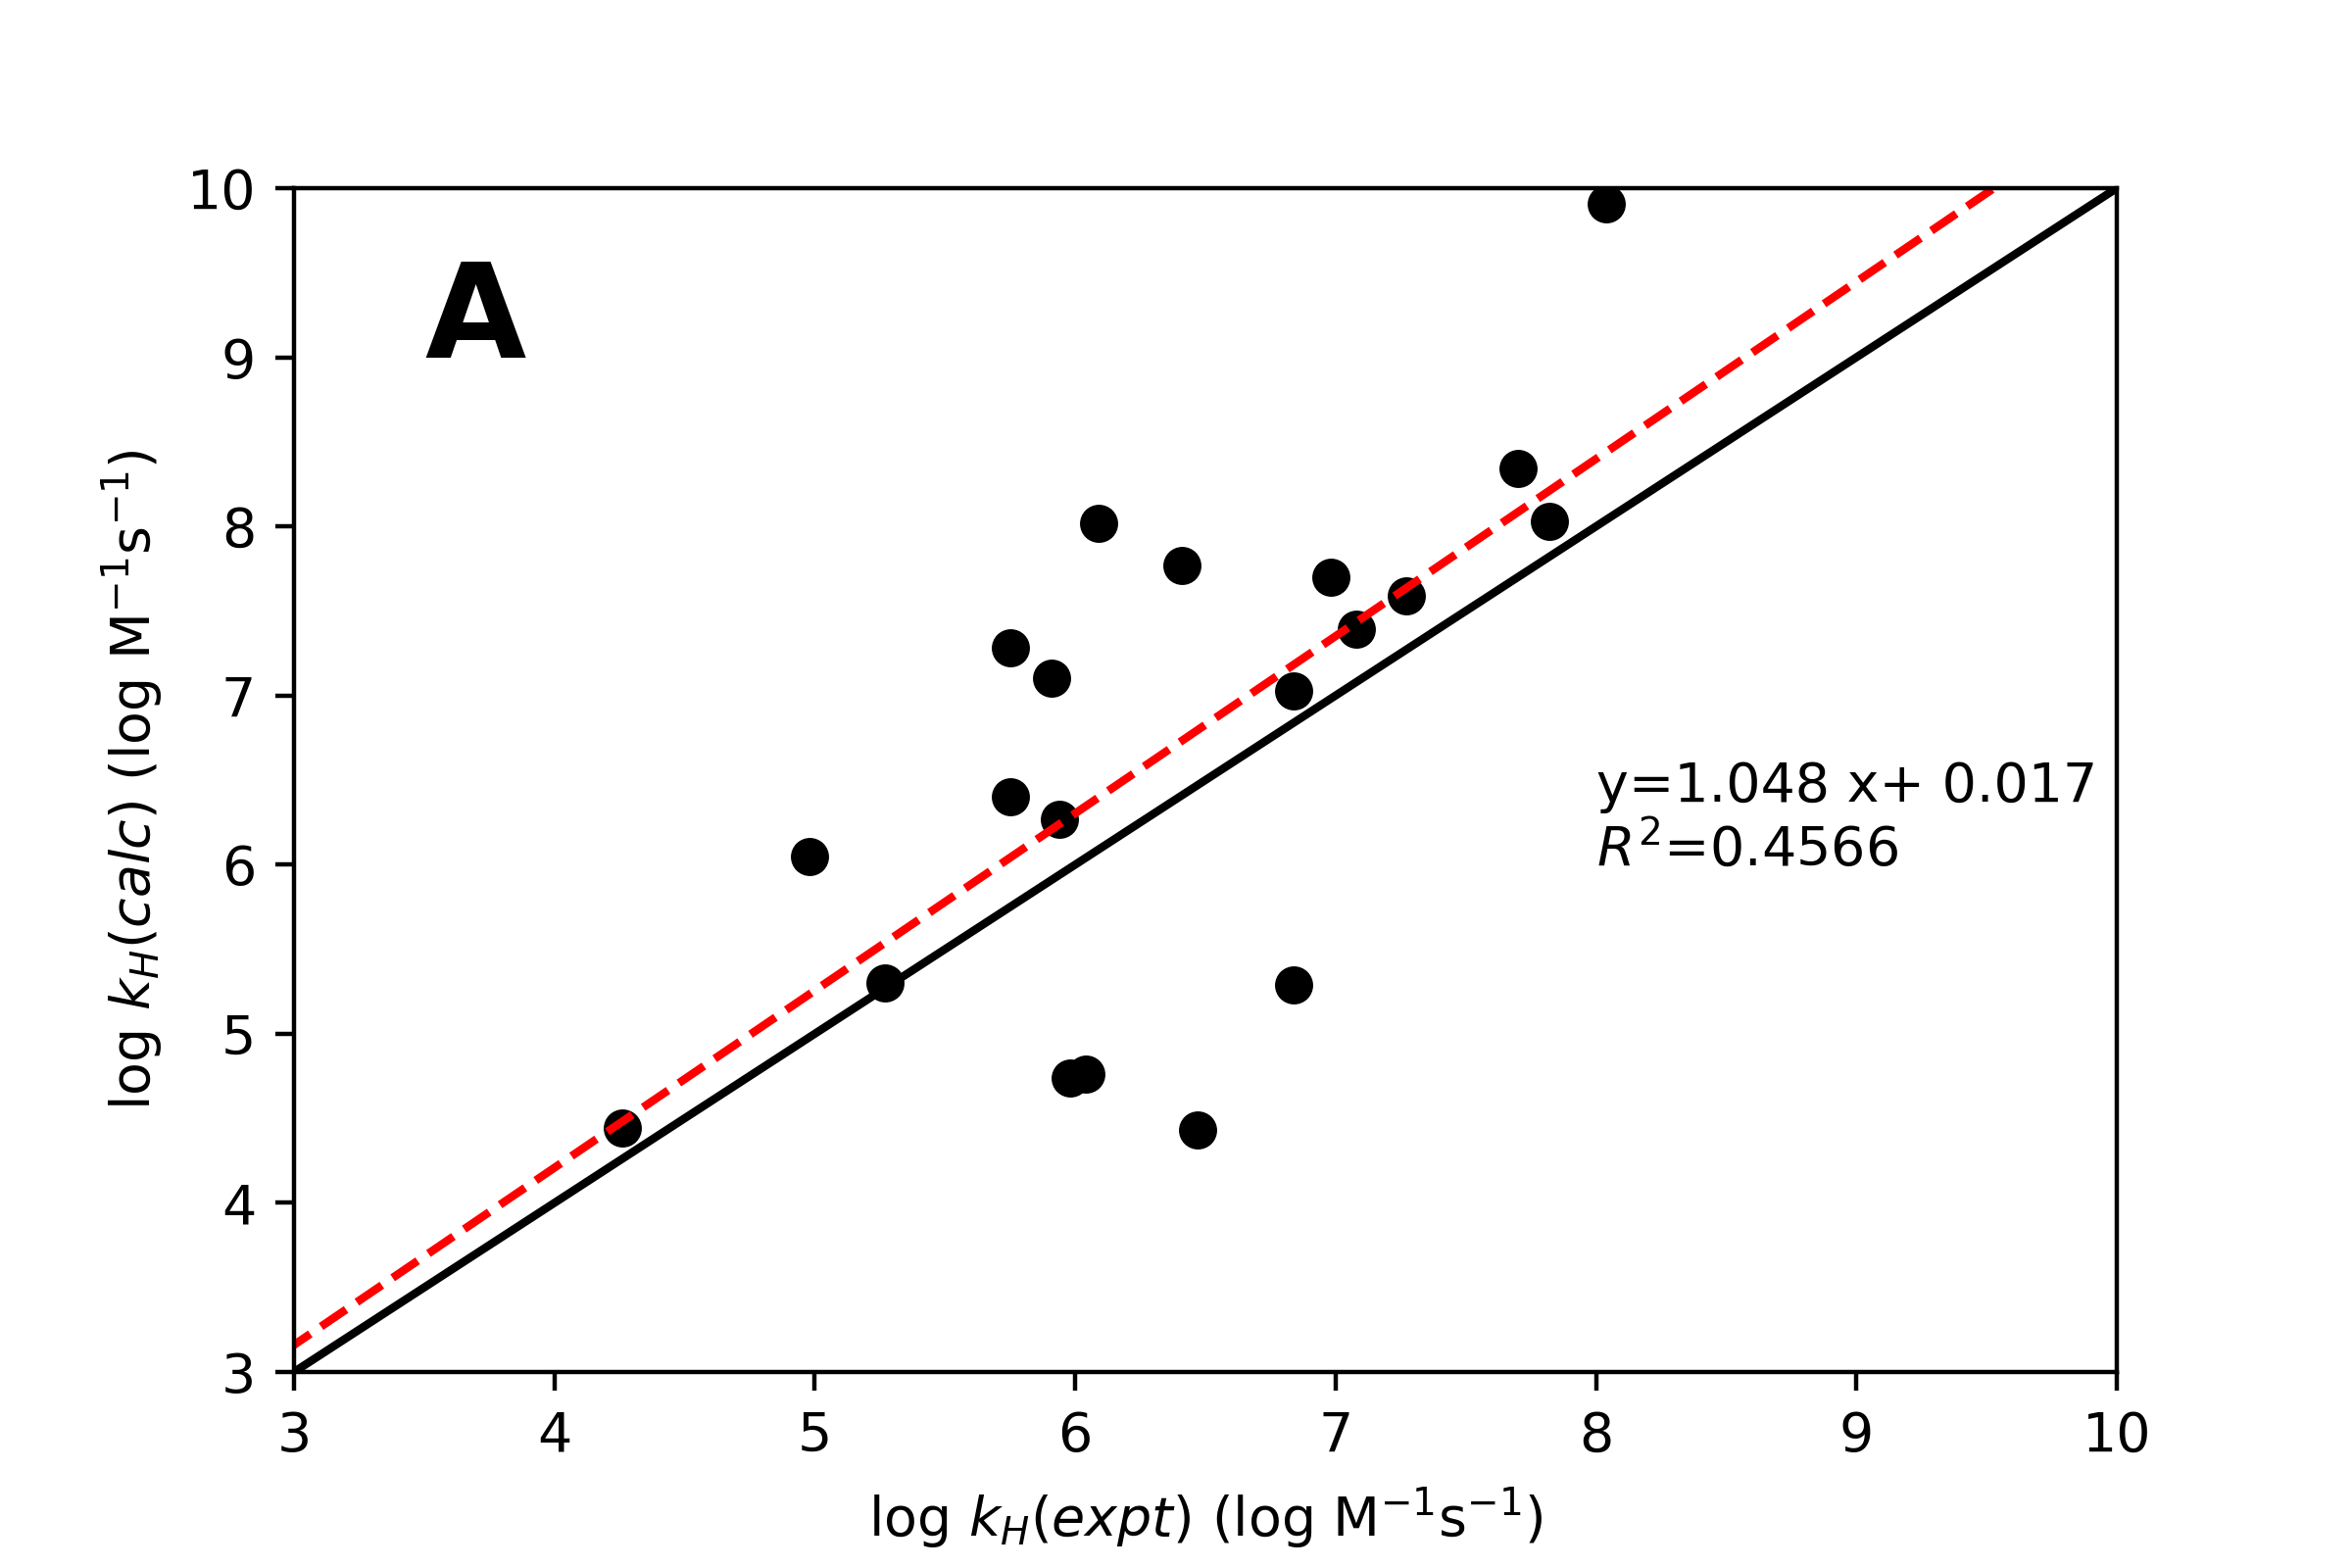
\includegraphics[width=\textwidth]{figures/kH-expt-gas}
\end{minipage}%
\begin{minipage}{8cm}
  \centering
  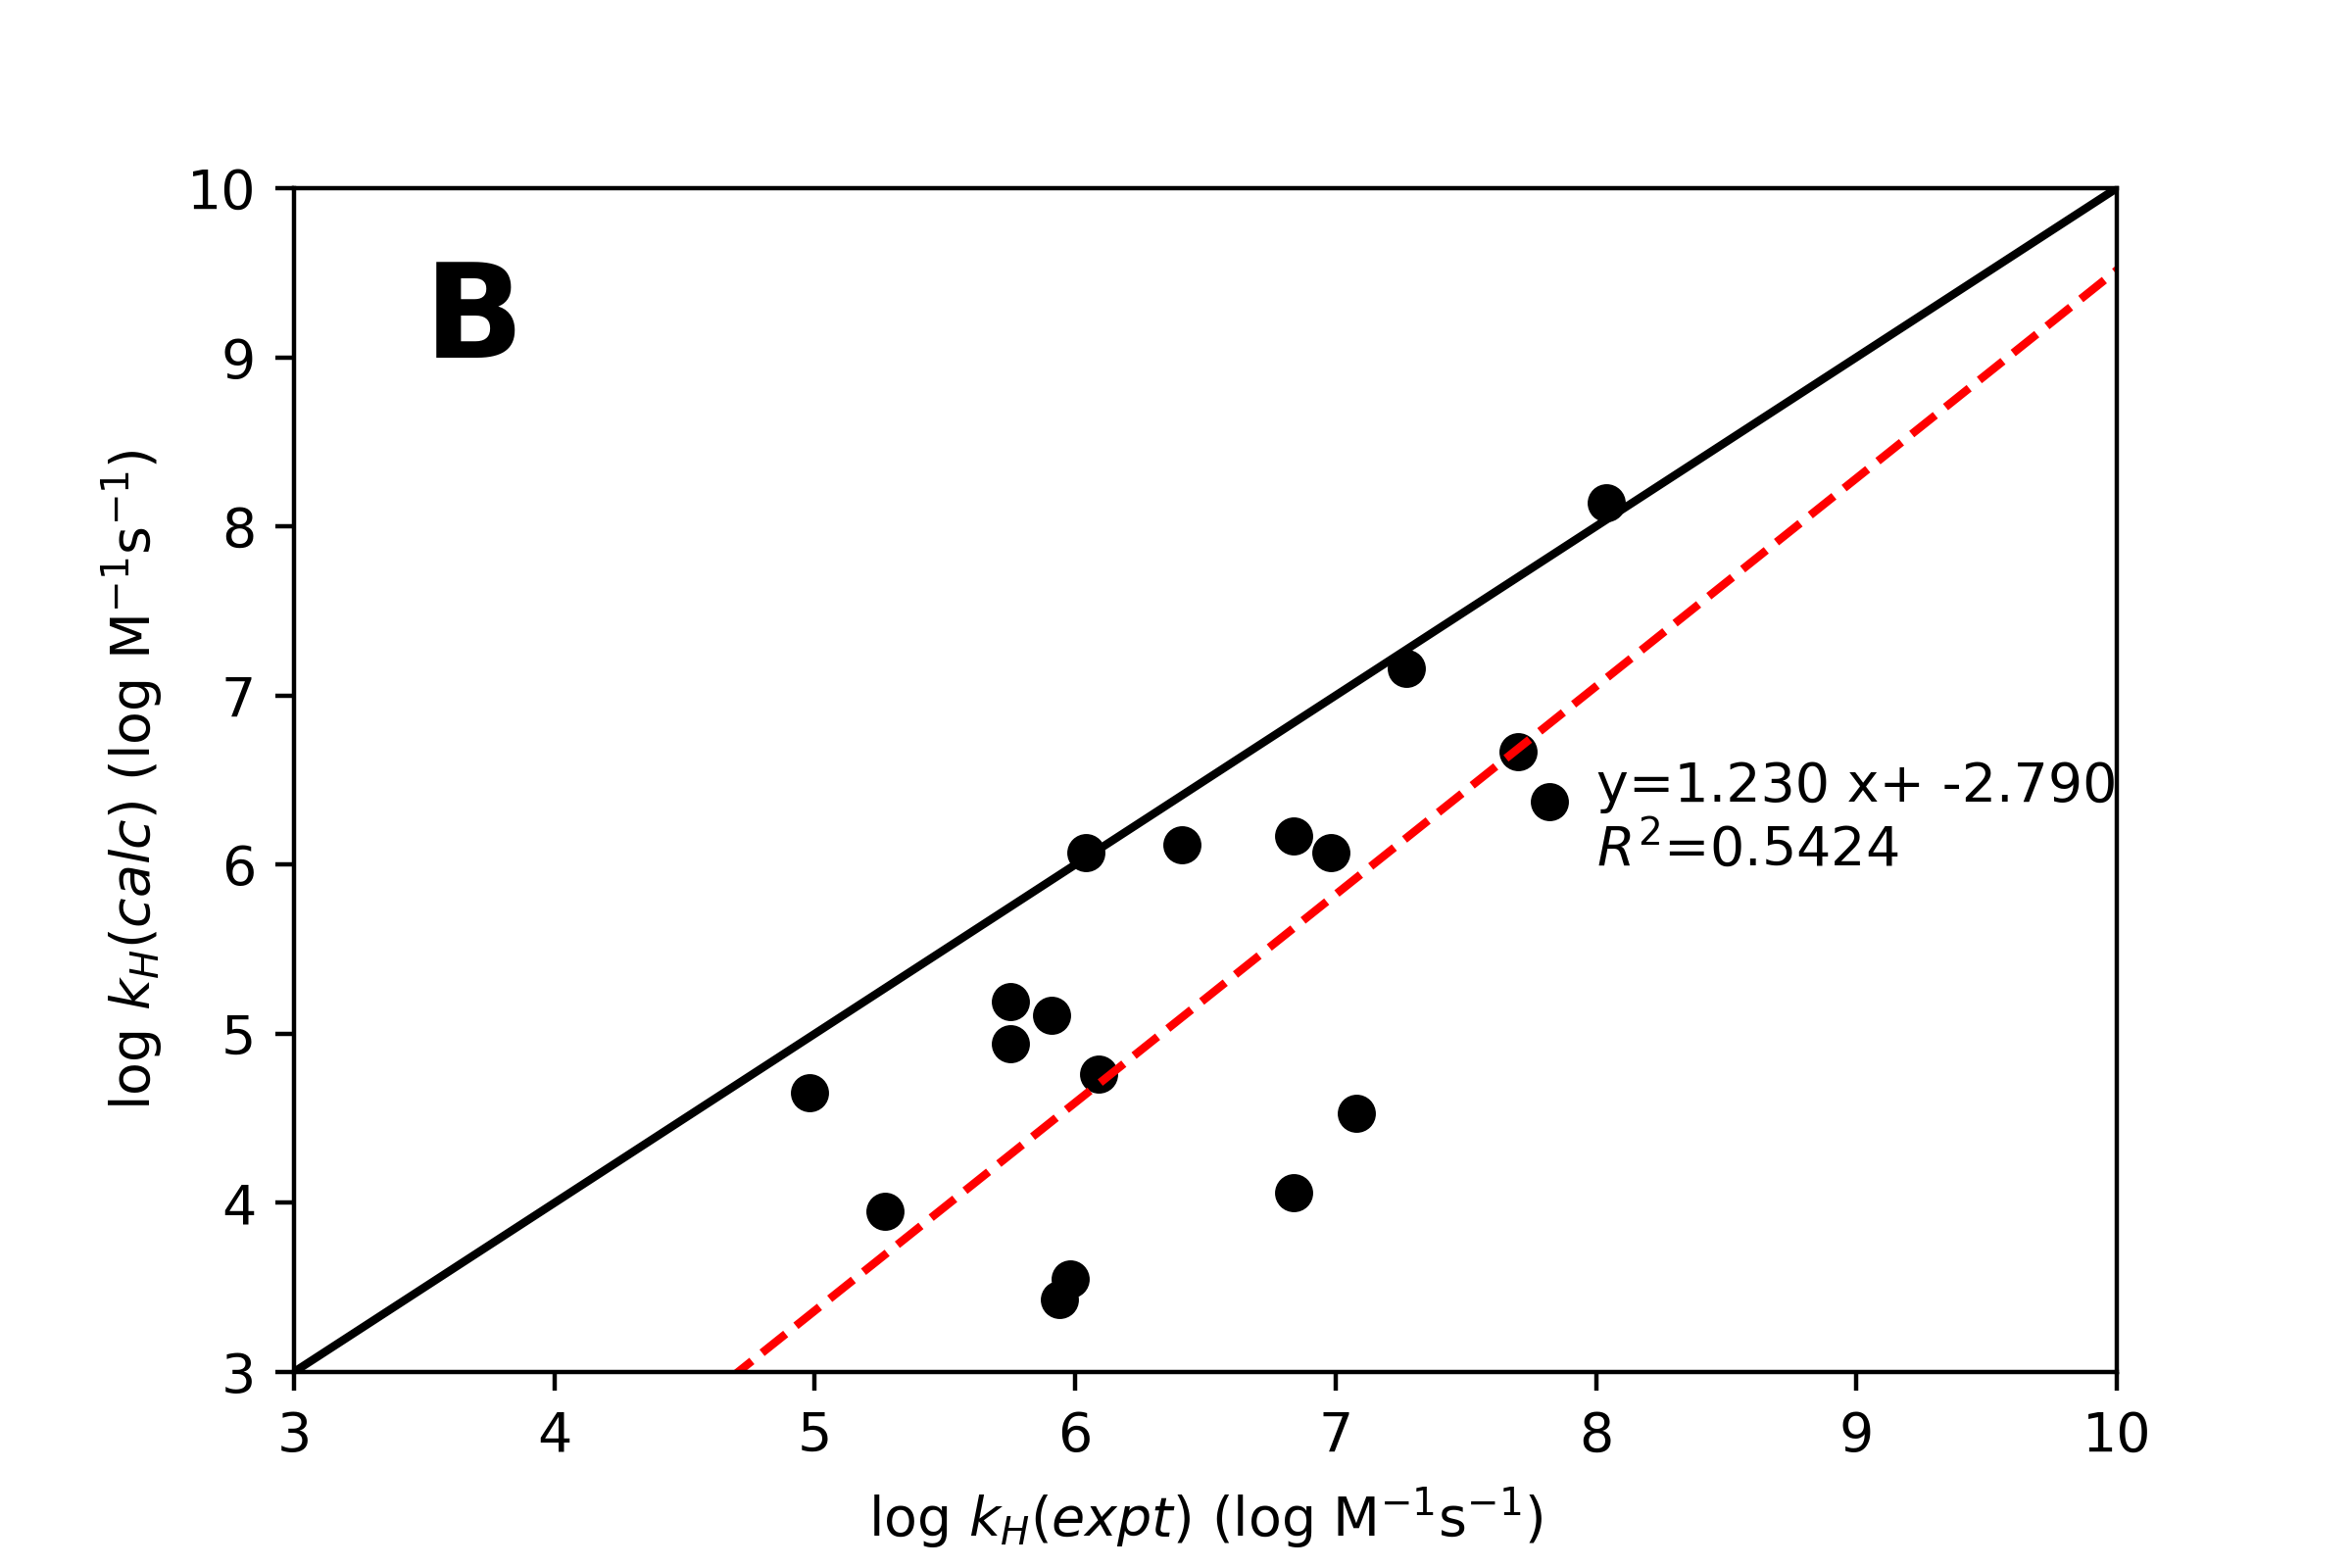
\includegraphics[width=\textwidth]{figures/kH-expt-mecn}
\end{minipage}
\caption[One-to-one plots comparing experimental and calculated rate constants
for HAT reactions between \cumo\ and various organic substrates.]{One-to-one
plots comparing experimental and \textbf{A} gas-phase calculated and \textbf{B}
solvent-phase rate constants for HAT reactions between \cumo\ and various
organic substrates.} \label{fig:ap-kH-comp}
\end{figure}

\chapter{Chapter~\protect\ref{ch:hat} Additional Data}\label{ap:hat}

\sectionmark{Benchmarking DFT based methods}
\section{Benchmarking DFT based methods for the binding of alkali and alkaline
earth metals to organic substrates and oxygen centred radicals}
\sectionmark{Benchmarking DFT based methods}
\label{sec:benchmark}

In order to be confident of the results of quantum mechanical mechanistic
studies, the method of choice must be calibrated. While DFT-based methods have
been widely applied to these studied, few studies have previously investigated
alkali and alkaline earth-metal cation binding to organic
substrates.\cite{Corral2003, Suarez2011, Siu2001, Baldauf2013} Most importantly,
benchmark quality data for a wide variety of metals binding to biologically
relevant substrates and oxygen-centred radicals does not exist to calibrate
DFT-based methods. Therefore, I performed a benchmark study which incorporated
all the biologically relevant alkali and alkaline earth-metal cations, models
for dipeptides including amino acid side chains, oxygen-centred radicals, and
solvents which are utilized in the experimental mechanistic studies involved in
probing these systems. Unfortunately, due to computational restrictions
(\emph{vide infra}), benchmark quality calculations on the originally proposed
benchmark set were not possible. Full details of the originally proposed
benchmark set are shown in~\ref{fig:ap-set1}.

\begin{scheme}[!htbp]
  \centering
    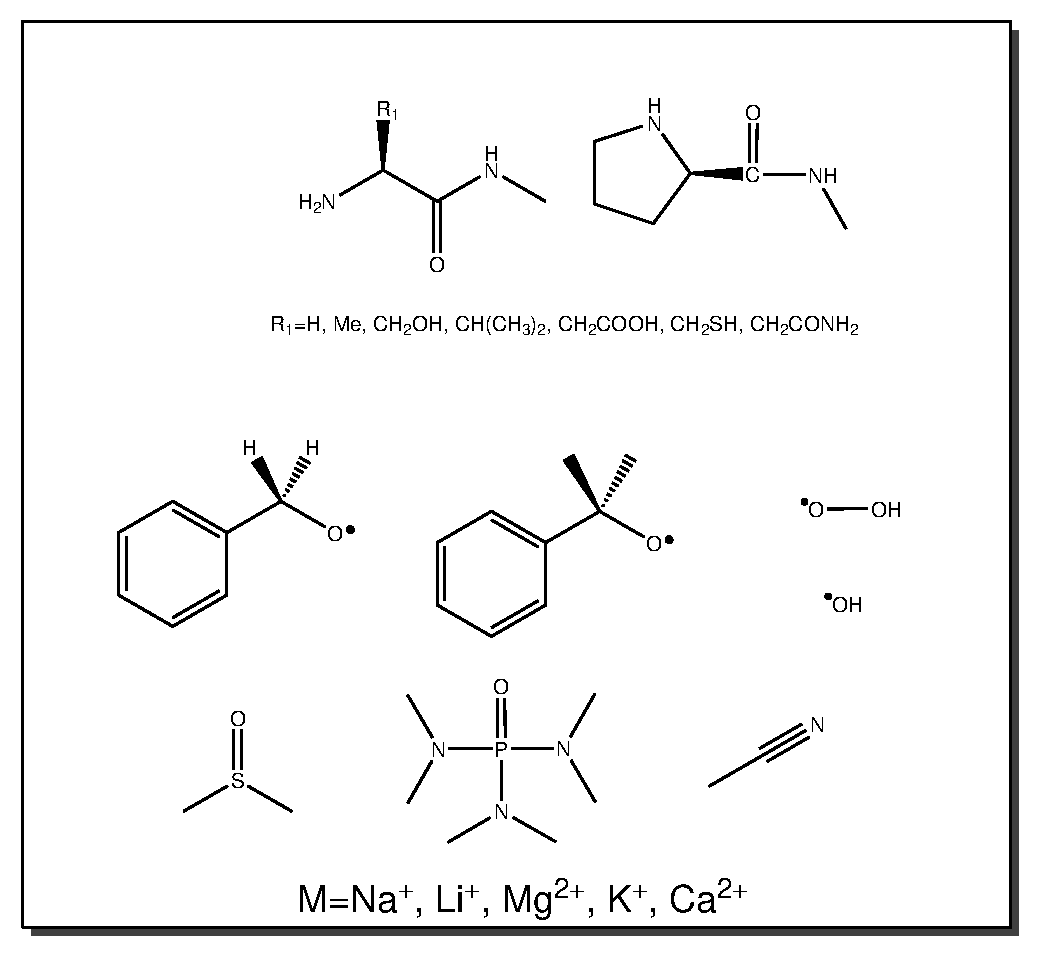
\includegraphics[width=\textwidth]{figures/set1.eps}
    \caption[Initial proposed benchmark set of substrates/radicals and metal
    cations.]{Initial proposed benchmark set of substrates/radicals and metal
    cations. Note this set consists of all combinations of substrates and metal
    cation, thus there are 75 complexes in the set. Conformational analysis
    using the Hyperchem package\cite{Hyperchem16} to identify the lowest energy
    conformers of all the substrates was completed using the AM1 semi-empirical
    approach. Geometry optimizations were then performed without metal cations
    at the LC-$\omega$PBE-D3(BJ)/6-31+G(2d,2p) level of theory. Several binding
    sites were investigated and optimized at the same level of theory.
    Benchmark quality structures have been optimized at the
    LC-$\omega$PBE-D3(BJ)/6-311+G(3df,3pd) level of theory. I am awaiting
    computational resources to performed CCSD(T)-F12$^*$/Def2-QZVPPD
    calculations.} \label{fig:ap-set1}
\end{scheme}

Benchmark quality binding energies are generally calculated using the ``gold
standard'' approach, CCSD(T)/CBS, where correlation consistent basis
sets\cite{Marshall2011, Rezac2013} (cc-pV\emph{X}Z, \emph{X}=T,Q,5) developed by
Dunning and\cite{Vydrov2006, Vydrov2006a} co-workers are used for complete basis
set extrapolation. For the alkali and alkaline earth-metals, \citet{Iron2003}
demonstrated that additional $d$-type basis functions are necessary to obtain
reasonable results. It is also necessary to include core-correlation of at least
the first core shell in alkali and alkaline earth metals, thus it would be
appropriate to use core valence basis sets such as
cc-pCV$X$Z.\cite{Peterson2002} \citet{Iron2003} also developed core-valence
basis sets for the alkali and alkaline earth-metals, however I was not able to
obtain these basis sets until very recently.\footnotemark These basis sets
should be considered for future benchmarking work. Given these difficulties, I
originally chose the augmented version of the polarization consistent basis sets
of Jensen and co-workers\cite{Jensen2001, Jensen2002, Jensen2002a, Jensen2003}
(aug-pc-\emph{N}, \emph{N}=2,3,4), which have been shown to converge to the CBS
limit systematically\cite{Kupka2007} and are available for all the elements of
interest.

\footnotetext{See http://theochem.weizmann.ac.il/web/papers/group12.html for the
CV$N$Z basis sets for Li, Be, Na, Mg, K, Ca.}

While performing CCSD(T)/CBS calculations, I observed that the metal cations
(and neutral metal atoms), did not converge smoothly to the complete basis set
limit. As a consequence, complete basis set extrapolation is not feasible. In
light of this problem, I decided to re-evaluate the size scope of the benchmark
set being used. In order to facilitate future DFT-based work and probe the issue
of basis set convergence of alkali and alkaline earth metals, a benchmark set of
small substrates was proposed. This new set is shown in \ref{fig:set2}. The new,
small benchmark set was selected to include important functional groups and
radicals found in biological systems, and one of the most common solvents used
in physical organic experiments, acetonitrile.

\begin{scheme}[!htbp]
  \centering
    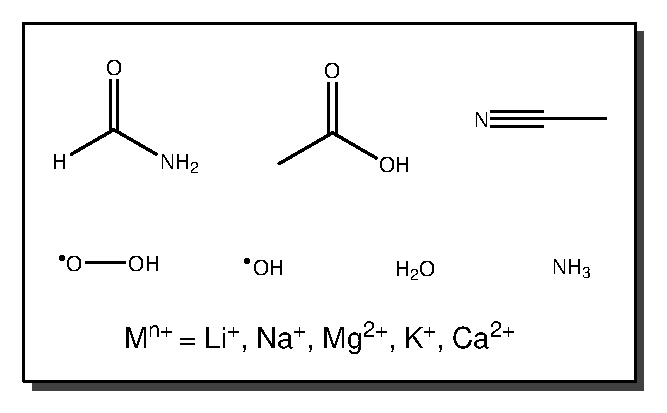
\includegraphics[width=\textwidth]{figures/set2.eps}
    \caption{Revised benchmark set of small substrates and cations. Note this
    set consists of all combinations of substrates and metal cations, i.e.,
    there are 35 complexes in the set.} \label{fig:set2}
\end{scheme}

\subsection{Metal cation basis set convergence}

In order to perform complete basis set (CBS) extrapolation, the total energy of
a molecule/atom should converge smoothly to the CBS limit.\cite{Truhlar1998}
However, CCSD(T,Full)/aug-pc$N$ ($N$=1,2,3,4) calculations for alkali and
alkaline earth-metals convergence of poorly to the CBS limit
(See~\ref{fig:ap_pes_metals}). Examining the energy of each ion relative to the
smallest basis set, for \ch{Li^+} the value appears to converge reasonably,
however this is because there are only 2 electrons in this ion. For all of
\ch{Na^+}, \ch{Mg^{2+}}, \ch{K^+}, and \ch{Ca^{2+}}, there appears to be no
convergence to the CBS limit as no asymptote is reached. This is problematic as
it means that CBS extrapolation would result in a significant degree of
uncertainty in the estimated CBS limit total energy.

\begin{figure}[!htbp]
  \centering
    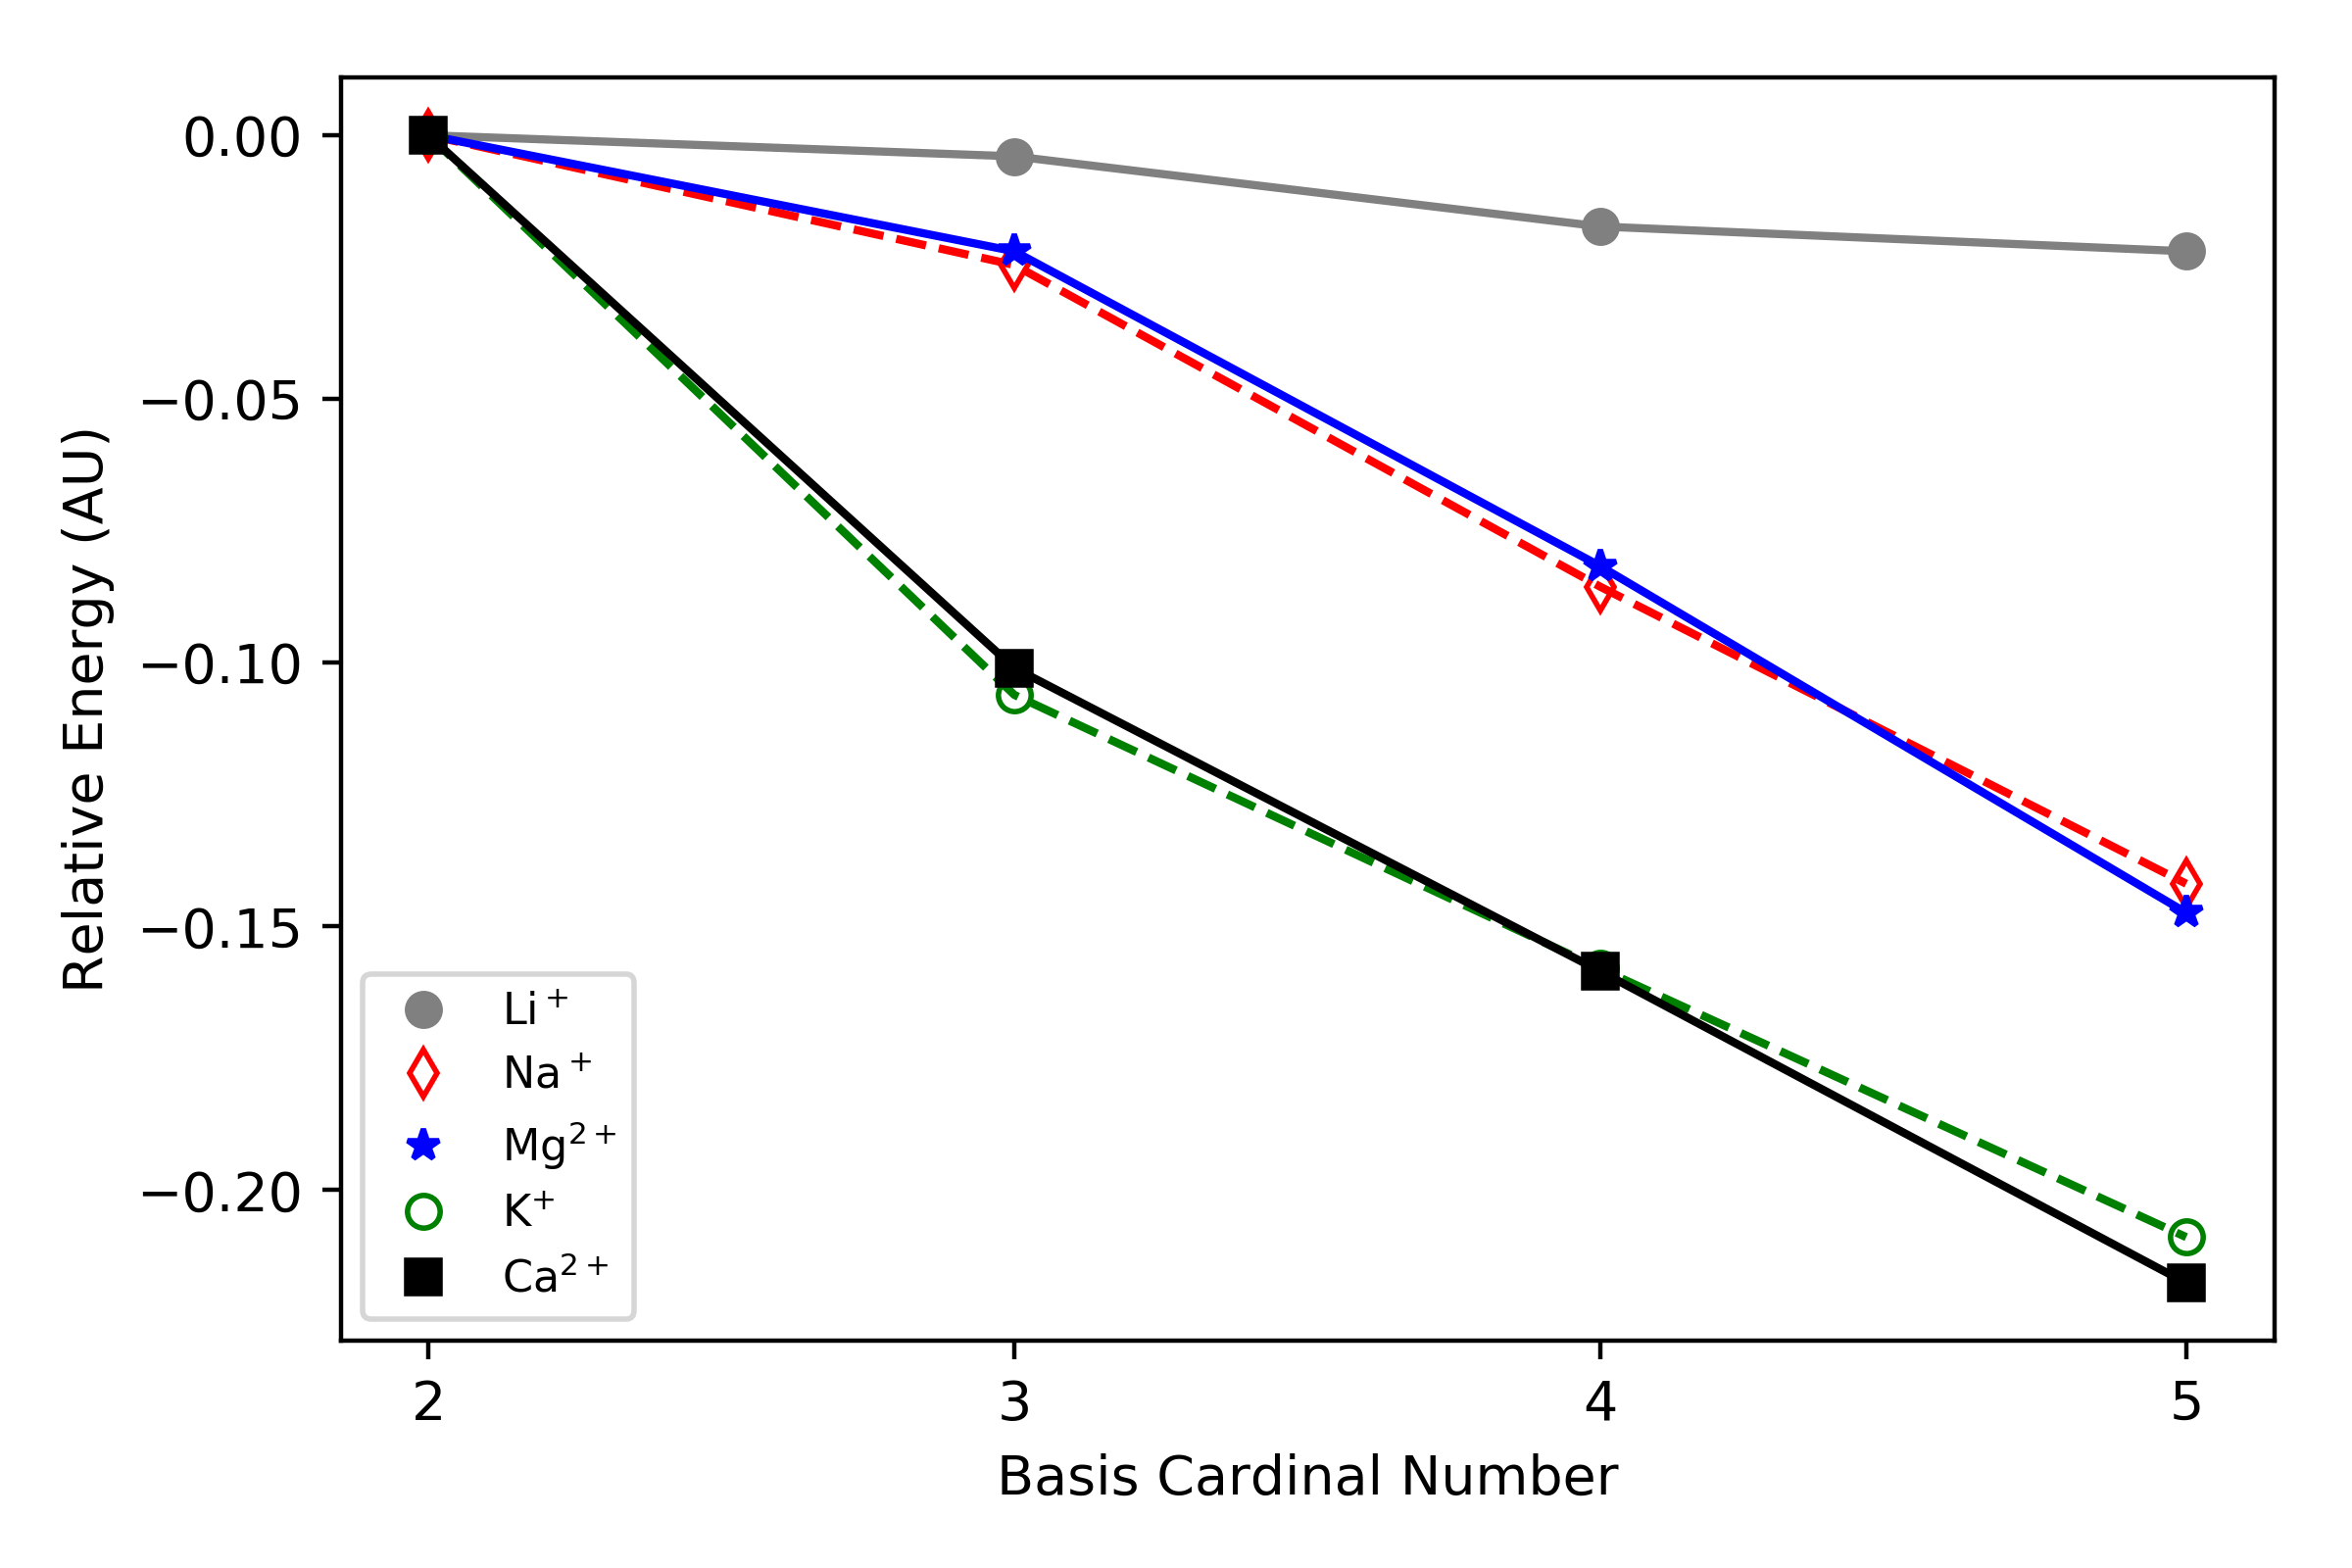
\includegraphics[width=\textwidth]{figures/pes_metals}
    \caption[Basis set convergence for alkali and alkaline earth-metal
    cations.]{Basis set convergence of CCSD(T,Full)/aug-pc-$N$ ($N$=1,2,3,4)
    for alkali and alkaline earth-metal cations. The relative energy of each
    basis set relative to the aug-pc-1 for each metal. The cardinal number of
    the aug-pc-$N$ basis sets is $X=N+1$.} \label{fig:ap_pes_metals}
\end{figure}

The poor convergence was thought to be a result of poorly suited basis sets to
full core-correlation. However, the same CCSD(T,Full) calculations using the
core-correlation (cc-pCV$N$Z) basis sets also show unsatisfactory convergence
for \ch{Na^+} and \ch{Mg^{2+}} (See~\ref{fig:ap_pes_metals_2}). Therefore, I was
tasked with finding a method which would give results which best approximate
alkali and alkaline metal binding at the complete basis set limit. I decided to
use an explicitly correlated CCSD(T) treatment known as ``F12$^*$'' to more
rapidly approach the CBS limit.\cite{Tenno2012} I tested both the
core-correlation consistent basis set developed for used with explicitly
correlation (cc-pCV$X$Z-F12),\cite{Peterson2008} and the Ahlrich basis sets
(Def2-SVP,-TZVPPD, and -QZVPPD).\cite{Rappoport2010} Both these basis sets
combined with the CCSD(T,Full)-F12$^*$ methodology gave satisfactory convergence
to the CBS limit for the sodium and magnesium ion
(See~\ref{fig:metals_explicit}) for the convergence of all metal ions calculated
with the CCSD(T,Full-F12$^*$/Def2-QZVPPD method). Given that Def2-QZVPPD is
available for almost every atom on the periodic table, and the observed
convergence to the CBS limit, this basis set was selected for benchmark quality
binding energies.

\begin{figure}[!htbp]
  \centering
    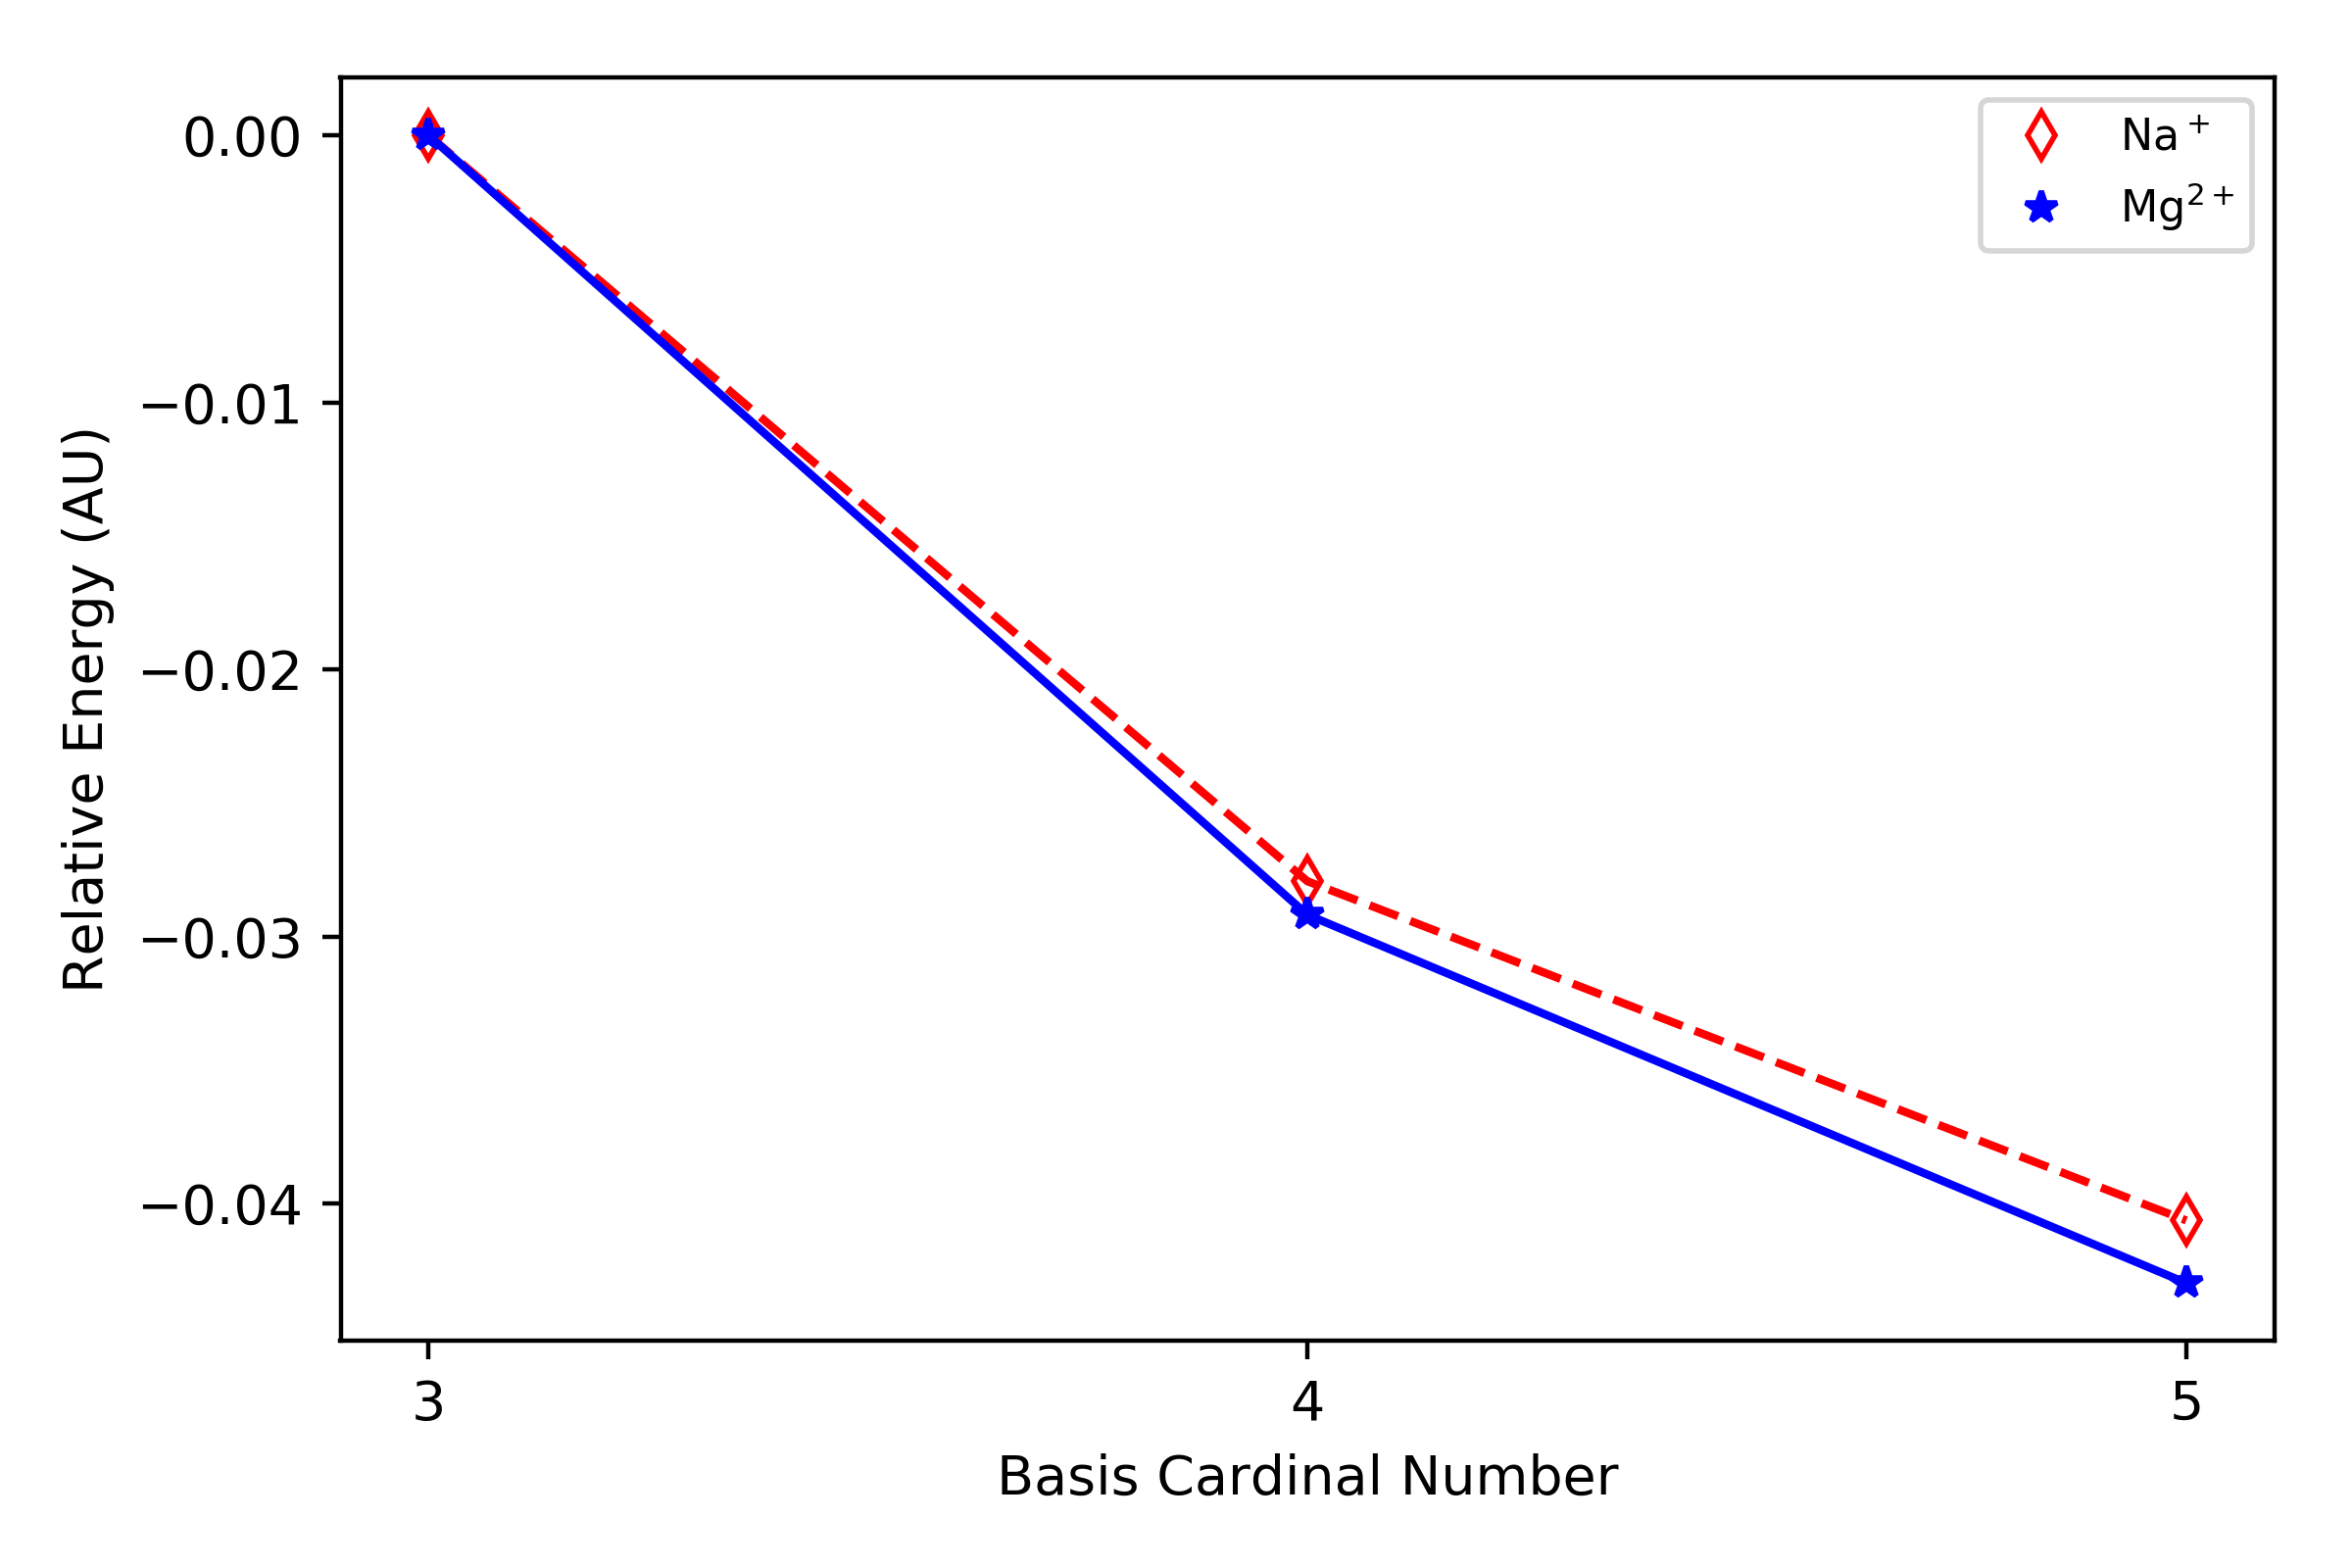
\includegraphics[width=\textwidth]{figures/ap_pes_metals}
    \caption[Basis set convergence for sodium and magnesium ions with
    core-correlation basis sets.]{Basis set convergence of
    CCSD(T,Full)/cc-pVC$X$Z ($X$=3,4,5) for sodium and magnesium ions. The
    relative energy of each basis set relative to the cc-pVCDZ for each metal.
    The cardinal number of the basis sets is $X$.} \label{fig:ap_pes_metals_2}
\end{figure}

\begin{figure}[!htbp]
  \centering
    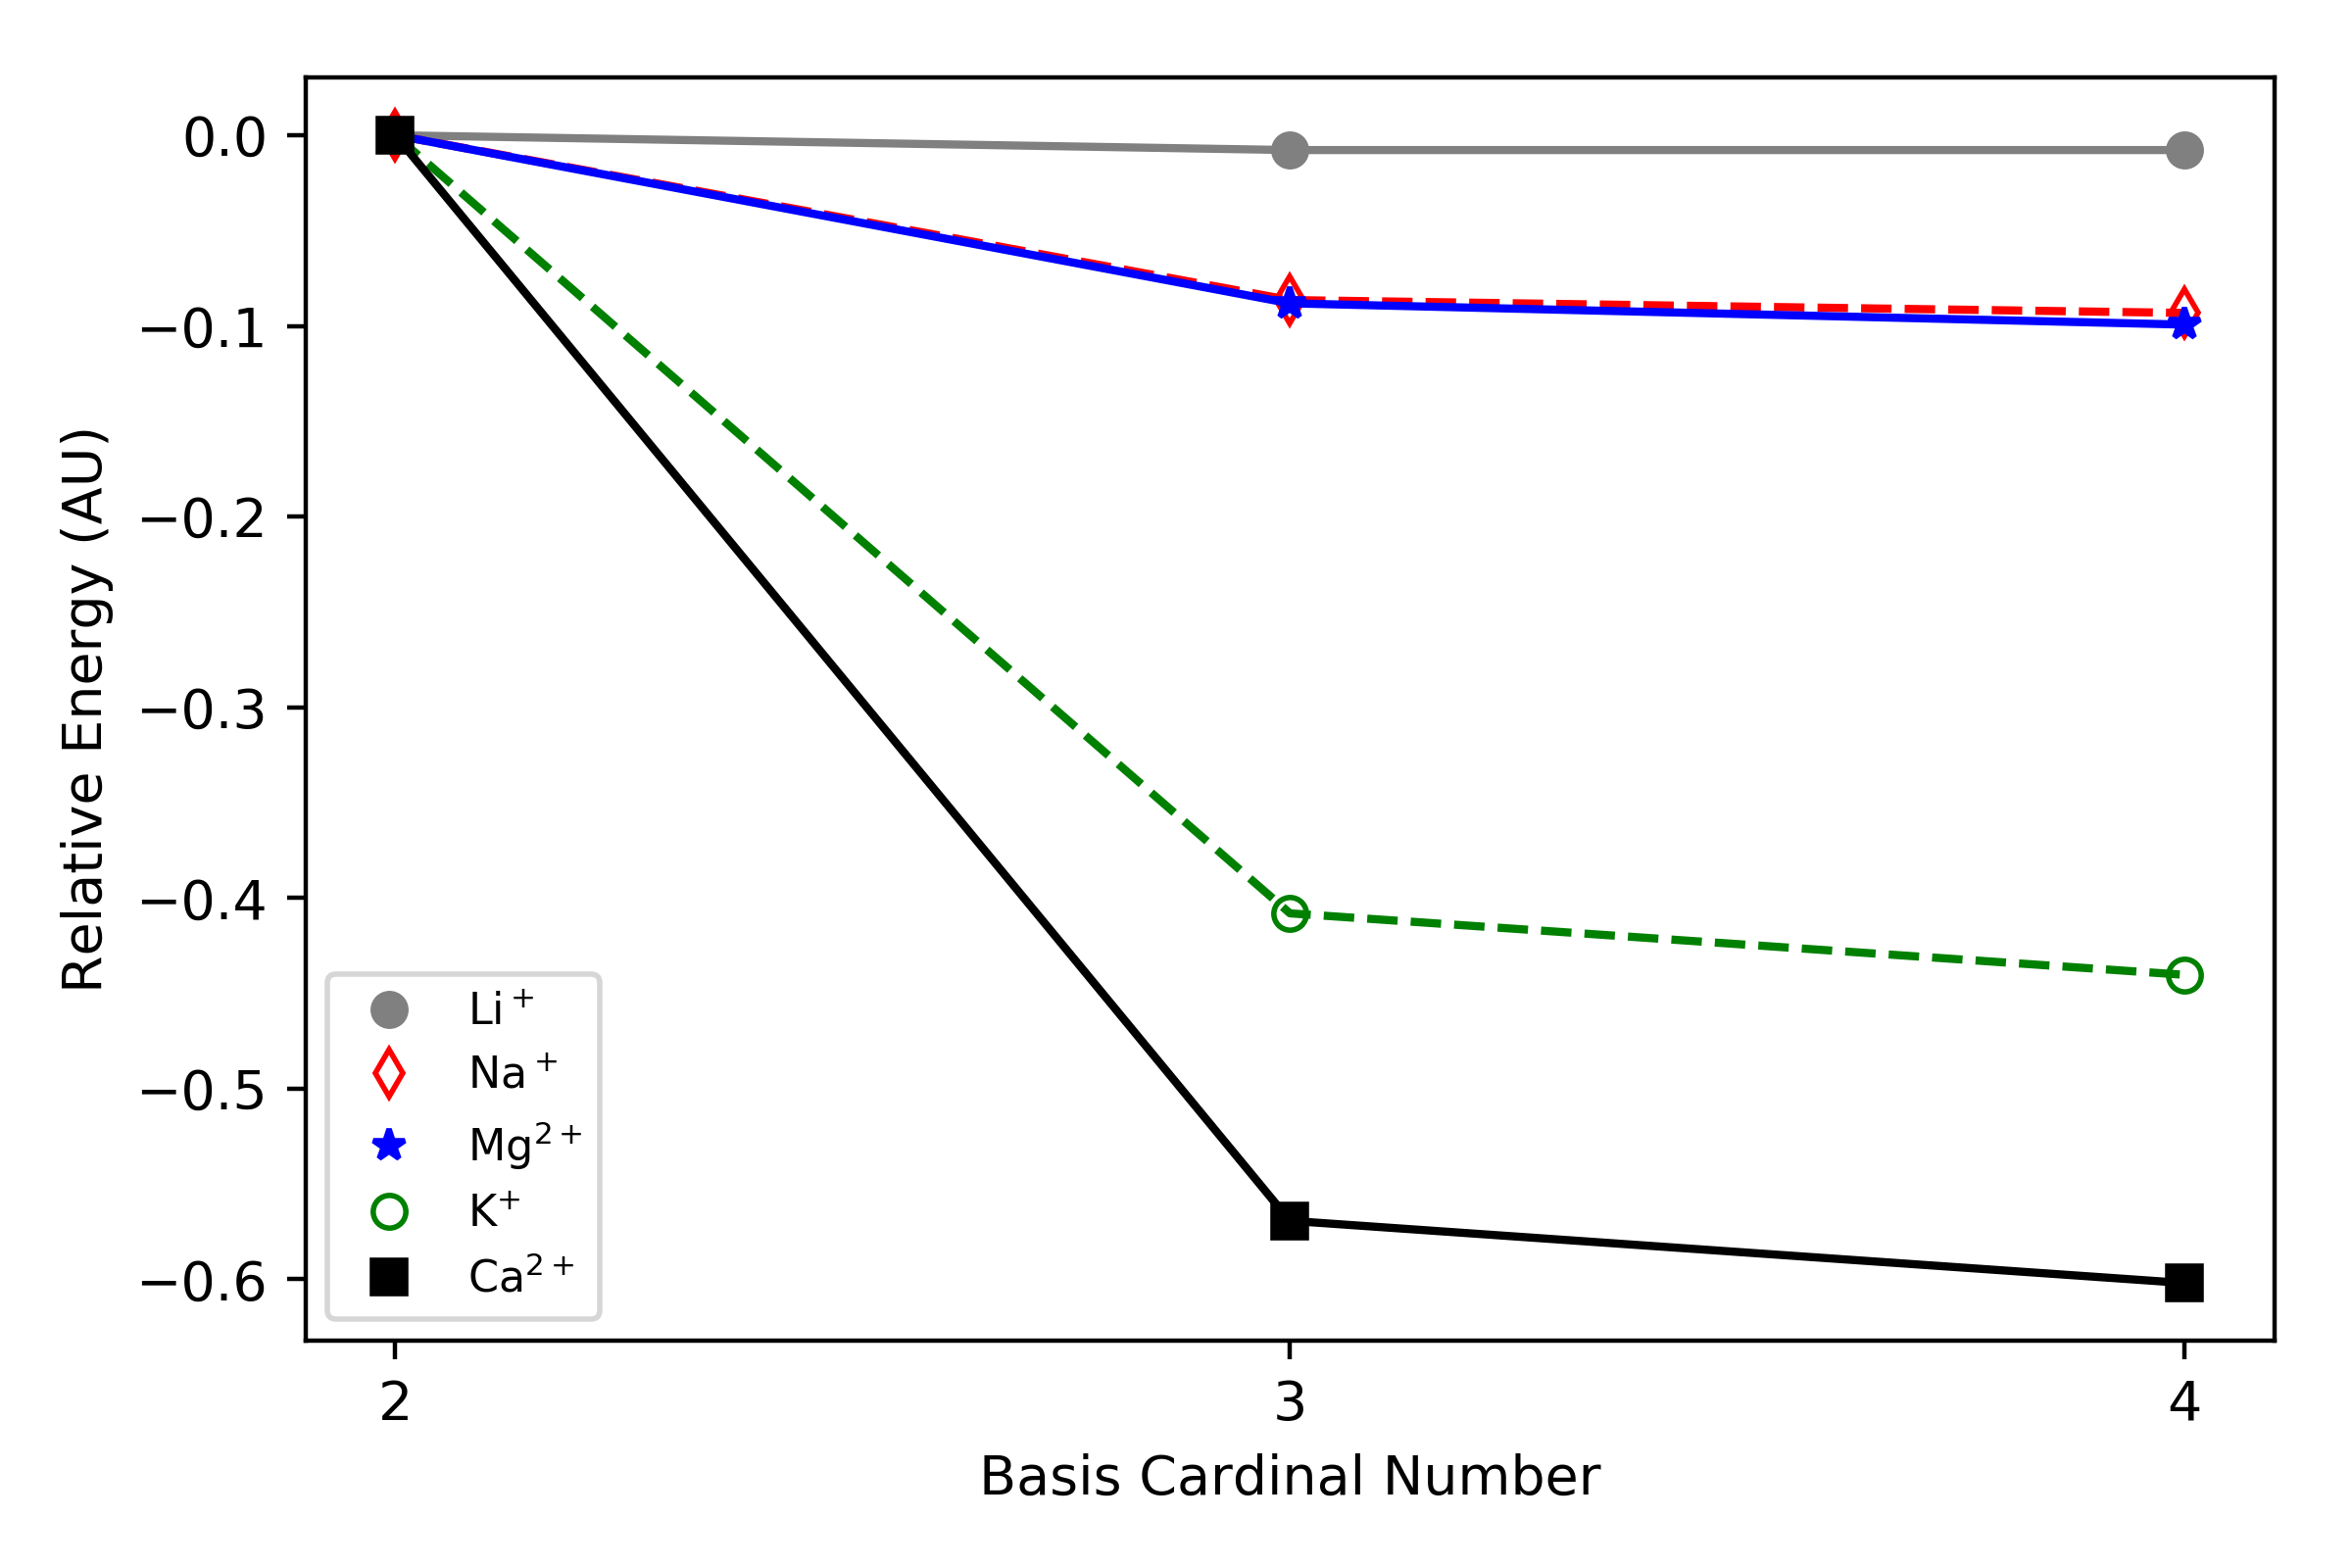
\includegraphics[width=\textwidth]{figures/ap_metals_explicit}
    \caption[Explicitly correlated basis set convergence for alkali and
    alkaline earth-metal cations.]{Explicitly correlated
    CCSD(T,Full)-F12$^*$/Def2-$X$ ($X$=SVP,TZVPPD,QZVPPD) basis set convergence
    for alkali and alkaline earth-metal cations. The relative energy of each
    basis set relative to the Def2-SVP for each metal. The cardinal number of
    the basis sets is $X$.} \label{fig:metals_explicit}
\end{figure}

To the best of my knowledge, there is no precedent for extrapolating the Ahlrich
basis sets, thus the final benchmark energies are at the
CCSD(T)-F12$^*$/Def2-QZVPPD level of theory, without extrapolation. The
convergence of the total energies of the cations can be estimated as the sum of
the experimental ionization energies of the ions. These results are listed
in~\ref{tab:metal-energy}. The calculated values are too high (i.e., not at the
CBS limit), and deviate from experiment from 0.16 and 0.66 AU (4.4--18 eV).
Deviations of this magnitude are rather significant, and are likely due to the
increasing contribution of ``relativistic effects'' with increasing atomic
number. Additionally, there may be cumulative experimental error, as the
experimental ionization energies range from 4--5500 eV. Relativistic effects
were not considered herein, thus, the calculated binding energies herein are
likely the best available approximation to the non-relativistic gas-phase
metal-substrate binding energy.

\begin{table}[!htbp]
  \caption[Total energy of alkali and alkaline earth-metal cations.]{Total
  energy of alkali and alkaline earth-metal cations from experimental
  ionization energies\cite{CRC2016} (Expt.) and calculated (Calc.) at the
  CCSD(T,Full)-F12$^*$/Def2-QZVPPD level of theory. All values are in units of
  AU.} \label{tab:metal-energy}
  \begin{tabular}{l c c}
    \textbf{Ion} & \textbf{Expt.} & \textbf{Calc.} \\
    \hline
    \ch{Li^+} & -7.47798 & -7.27983 \\
    \ch{Na^+} & -162.43089 & -162.24203 \\
    \ch{Mg^{2+}} & -200.32523 & -199.49171 \\
    \ch{K^+} & -601.93332 & -601.77381 \\
    \ch{Ca^{2+}} & -680.19158 & -679.53065
  \end{tabular}
\end{table}

\subsection{High level results and evaluation of various density-functional theory based methods}

\ref{tab:ccsd-metal} lists the benchmark binding energy values calculated at the
CCSD(T,Full)-F12$^*$/Def2-QZVPPD//LC-$\omega$PBE-D3(BJ)/6-311+G(3df,3pd) level
of theory. Some general trends are that alkaline earth-metals bind more strongly
than alkali earth-metals. Also, the order of binding follows the Lewis acidity
of the metal ions: \ch{Mg^{2+}} $>$ \ch{Ca^{2+}} $>$ \ch{Li^+} $>$ \ch{Na^+} $>$
\ch{K^+}. The metals all appear to bind most strongly to the amidic
oxygen-centre, reflecting the higher Lewis basicity. The metals also bind
weakest to the oxygen-centred radicals, with greater binding to \ch{HOO^.} as
compared to \ch{HO^.}.

\begin{table}[!htbp]
  \caption[Benchmark gas-phase binding energies of alkali and alkaline
  earth-metals with small organic substrates and radicals.]{Benchmark gas-phase
  binding energies of alkali and alkaline earth-metals with small organic
  substrates and radicals. Values are calculated at the
  CCSD(T,Full)-F12$^*$/Def2-QZVPPD//LC-$\omega$PBE-D3(BJ)/6-311+G(3df,3pd)
  level of theory. All values are in \kcalmol.}\label{tab:ccsd-metal}
  \begin{tabular}{l c c c c c}
            &\ch{Li^+}&\ch{Na^+}&\ch{Mg^{2+}}&\ch{K^+}&\ch{Ca^{2+}}\\
    \hline
    \ch{H2O}    & -34.7 &  -24.4 &  -82.0  &  -17.8 &  -56.8 \\
    \ch{NH3}    & -39.9 &  -28.2 &  -98.1  &  -19.8 &  -65.3 \\
    MeCN        & -44.4 &  -33.0 &  -113.1 &  -24.9 &  -80.7 \\
    Formamide   & -50.7 &  -36.9 &  -128.2 &  -28.5 &  -96.1 \\
    Formic acid & -38.4 &  -27.0 &  -101.9 &  -20.0 &  -72.6 \\
    \ch{HO^.}   & -21.3 &  -16.8 &  -57.0  &  -12.4 &  -40.7 \\
    \ch{HOO^.}  & -27.1 &  -19.1 &  -72.2  &  -13.9 &  -49.0
  \end{tabular}
\end{table}

Next, 31 DFT-based methods combined with a moderate basis set (6-31+G(2d,2p))
and a large basis set (6-311+G(3df,3pd)) were tested for their ability to
estimate the binding energy between metal cations and substrates. The mean
absolute/signed errors (MAE/MSE) and maximum and minimum errors for each method
are listed in~\ref{tab:dft-metal}.

\setlength\LTleft{-1cm}
\begin{longtable}[!htbp]{m{4cm} c c | c c}
\caption[Evaluation of DFT-based methods for alkali and alkaline metal binding
to organic substrates and radicals.]{Evaluation of DFT-based methods for alkali
and alkaline metal binding to organic substrates and radicals. All values are
in \kcalmol. Negative values indicate under-binding.} \label{tab:dft-metal}\\
\textbf{Method}&\textbf{MAE/MSE}&\textbf{Max./Min}&\textbf{MAE/MSE}&\textbf{Max./Min.}\\
\hline
 & \multicolumn{2}{c|}{6-311+G(3df,3pd)} & \multicolumn{2}{c}{6-31+G(2d,2p)}\\
B3\cite{Becke1993}LYP\cite{Lee1988} &  1.49/1.35 &  5.12/-0.57  &  1.59/-0.17 &  4.67/-7.28 \\
B3P86\cite{Perdew1986} &  0.94/0.47 &  3.87/-0.96  &  1.36/-1.08 &  1.99/-7.38 \\
B3PW91\cite{Perdew1991}  &  0.95/-0.14 &  2.74/-1.64  &  1.89/-1.70 &  1.47/-8.76 \\
BH+H\cite{Becke1993a}LYP &  1.89/1.84 &  5.29/-0.59  &  1.93/0.63 &  4.65/-5.64 \\
B\cite{Becke1988}LYP  &  1.60/1.07 &  5.56/-1.51  &  1.88/-0.75 &  5.30/-8.80 \\
BMK\cite{Boese2004}   &  0.90/-0.70 &  1.13/-2.40  &  1.98/-1.93 &  0.86/-8.75 \\
BP86              &  1.63/-0.25 &  4.61/-3.21  &  2.27/-2.14 &  1.55/-9.38 \\
CAM-B3LYP\cite{Yanai2004} &  2.40/2.40 &  6.25/ 0.21  &  1.98/1.04 &  5.82/-5.25 \\
LC-$\omega$PBE\cite{Vydrov2006, Vydrov2006a} &  0.78/0.58 &  2.95/-0.73  &  1.34/-0.74 &  2.19/-8.00 \\
M05-2X\cite{Zhao2006} &  1.11/1.11 &  3.21/ 0.15  &  1.24/-0.17 &  2.55/-5.75 \\
M06\cite{Zhao2008}    &  1.05/-0.62 &  2.36/-4.83  &  1.83/-1.63 &  1.76/-9.03 \\
M06-2X\cite{Zhao2008} &  1.13/1.13 &  3.68/ 0.11  &  1.26/-0.07 &  3.00/-6.63 \\
M06L\cite{Zhao2006b} &  1.52/-1.14 &  2.64/-6.94  &  2.55/-2.48 &  1.21/-11.2 \\
MOHLYP\cite{Schultz2005} &  2.30/-2.02 &  1.52/-5.40  &  4.04/-3.96 &  0.89/-15.2 \\
PBE0\cite{Adamo1999, Ernzerhof1999} &  1.22/1.18 &  4.19/-0.31  &  1.25/-0.34 &  3.30/-7.25 \\
PBE\cite{Perdew1996} &  1.70/1.46 &  6.09/-0.87  &  1.58/-0.46 &  4.68/-8.15 \\
TPSS\cite{Tao2003}   &  1.38/0.95 &  4.88/-1.12  &  1.60/-0.98 &  2.91/-8.12 \\
B97\cite{Becke1997}D3\cite{Grimme2010} &  1.50/0.47 &  5.94/-2.19  &  1.69/-1.37 &  2.67/-8.41 \\
$\omega$B97\cite{Chai2008a} &  0.61/0.23 &  2.13/-1.72  &  1.41/-0.97 &  1.78/-7.57 \\
$\omega$B97XD\cite{Chai2008} &  1.12/-0.94 &  1.02/-4.52  &  2.24/-2.21 &  0.65/-8.64 \\
HSEH1PBE\cite{Heyd2004, Heyd2005} &  1.30/1.29 &  4.28/-0.16  &  1.23/-0.23 &  3.45/-6.95 \\
B3LYP-D3(BJ)\cite{Grimme2010, Johnson2006} &  2.86/2.86 &  7.50/ 0.34  &  1.92/1.34 &  7.05/-4.33 \\
BLYP-D3(BJ)       &  2.89/2.88 &  8.40/-0.14  &  1.83/1.06 &  8.14/-5.30 \\
B3PW91-D3(BJ)     &  1.47/1.40 &  5.81/-0.44  &  1.02/-0.14 &  3.88/-5.69 \\
BMK-D3(BJ)        &  1.03/0.80 &  4.05/-1.06  &  1.02/-0.43 &  2.03/-5.49 \\
BP86-D3(BJ)       &  1.77/1.29 &  7.78/-1.05  &  1.26/-0.60 &  3.96/-6.19 \\
CAM-B3LYP-D3(BJ)  &  3.19/3.19 &  7.50/ 0.78  &  2.27/1.82 &  7.07/-3.54 \\
LC-$\omega$PDE-D3(BJ)& 1.47/1.46 & 4.07/-0.06 &  1.33/0.14 &  3.30/-6.15 \\
PBE0-D3(BJ)       &  1.92/1.92 &  5.37/ 0.20  &  1.33/0.40 &  4.47/-5.74 \\
PBE-D3(BJ)        &  2.24/2.23 &  7.57/-0.22  &  1.44/0.30 &  5.90/-6.67 \\
TPSS-D3(BJ)       &  2.03/1.99 &  6.93/-0.30  &  1.25/0.06 &  4.56/-6.03
\end{longtable}
\setlength\LTleft{0pt}
\setlength\LTright{0pt}

Given the magnitude of the gas-phase binding energies, the overall agreement
between the benchmark values and the DFT-based method values with both moderate
and large basis sets is very good. Interestingly, the application of the
empirical D3(BJ) dispersion correction systematically decreases agreement with
benchmark values as it increases over-binding. Also, going from moderate to
large basis sets systematically increases the predicted binding energies, as
indicated by an increase in MSE across the board. I chose three of the best
performing methods (BMK-D3(BJ), TPSS-D3(BJ), and M05-2X) and performed geometry
optimizations with moderate basis sets on the reference structures to determine
if the choice of method would significantly impact the minimum energy bound
structure. These results are listed in~\ref{tab:ccsd-metal-opt}.

\begin{table}
  \caption[Comparison of single point and relaxed binding energies for alkali
  and alkaline metal binding with DFT-based methods.]{Comparison of single point
  (SP on benchmark structure) and relaxed (optimized with method) binding
  energies for alkali and alkaline metal binding with DFT-based methods and
  6-31+G(2d,2p) basis sets. Mean absolute error (MAE) values are in \kcalmol\
  and average root mean squared deviation (RMSD)(Root mean square deviation was
  calculated using the Kabsch algorithm\protect\cite{Kabsch1976} as implemented
  in the rmsd package available on GitHub (Calculate RMSD for two XYZ
  structures, GitHub, http://github.com/charnley/rmsd, accessed Nov. 18, 2016))
  of geometry are in \AA.}
  \label{tab:ccsd-metal-opt}
  \begin{tabular}{l c c c}
    Method & MAE(SP) & MAE(Relaxed) & Average RMSD \\
    \hline
    BMK-D3(BJ) & 1.02 & 1.24 & 0.012 \\
    M05-2X & 1.24 & 1.17 & 0.020 \\
    TPSS-D3(BJ) & 1.25 & 1.21 & 0.026 \\
  \end{tabular}
\end{table}

For all the three methods tested, the average of the root mean square deviations
(RMSD) from reference structures are very small (0.012--0.026 \AA). For
BMK-D3(BJ), re-optimization of the structures results in a slight increase in
MAE, while for TPSS-D3(BJ) and M05-2X, the opposite is true. As a whole, it
seems that DFT-based methods are capable of predicting gas-phase binding
energies for alkali and alkaline metal ions with organic substrates and
radicals. M05-2X appears to be one of the best performing DFT-based methods.
Furthermore, M05-2X is recommended by the QM-ORSA\cite{Galano2013} method, which
outlines ``best principles'' for calculating accurate HAT rate constants in
solution. And finally, M05-2X was previously used by our group in the study of
the HAT reaction between DMSO and \bno,\cite{vanSanten2016} thus I have selected
this method for further study of the effects of alkali and alkaline earth metal
cations on the barrier heights of HAT reactions. Note also that M05-2X is a
hybrid density-functional with 56\% HF-exchange, and thus should not suffer
significantly from delocalization error.

\section{HAT reactions involving non-redox active metals}
\subsection{DMA + \ch{HO^.}}

I was unsuccessful in performing full optimization calculations in the presence
of the metal salt. However, the ``guess'' TS structures obtained by freezing the
hydrogen atom acceptor donor bonds (as described in the Chapter 5 section)
herein represent approximated transition state structures and therefore provide
an estimate of the effects of metal salts in a more biologically relevant model.
The calculated reaction barriers are presented in~\ref{tab:dma-oh}.

\begin{table}[!htbp]
\caption[Calculated free energy (enthalpy) barrier for direct HAT from different
\ch{C-H} bonds in DMA by \ch{HO^.}, with and without \ch{NaCl}.]{Calculated free
energy (enthalpy) barrier ($\Delta G(H)^\ddagger$, \kcalmol) for direct HAT from
different \ch{C-H} bonds in DMA by \ch{HO^.}, with and without \ch{NaCl}. The
change in barrier height ($\Delta \Delta G(H)^\ddagger$) is calculated relative
to the same abstraction site without the inclusion of \ch{NaCl}. All barrier
heights are relative to separated reactants (or complexed DMA-NaCl) and were
calculated at the M05-2X-SMD(MeCN)/6-311+G(2d,2p)//M05-2X/6-31+G$^{**}$ level of
theory. $^*$Indicates estimated barrier based on ``guess'' TS structure.}
\label{tab:dma-oh}
  \begin{tabular}{l l c c}
Reaction   & Abstraction Site &  $\Delta G(H)^\ddagger$ & $\Delta\Delta G(H)^\ddagger$ \\
\hline
DMA + \ch{HO^.} &  trans           &  8.9(0.0)            &                \\
            &  cis                &  7.9(-2.7)           &                    \\
            &  acetyl             &  9.9(0.5)            &                    \\
DMA-NaCl + \ch{HO^.}&  trans$^*$      &  13.1(1.3)           &  4.2(1.3)          \\
            &  cis$^*$                &  12.9(0.2)           &  5.0(2.9)          \\
            &  acetyl$^*$             &  16.6(2.0)           &  7.7(1.5)          \\
  \end{tabular}
\end{table}

For the direct HAT reaction between \ch{OH^.} and DMA abstraction occurs
primarily from the cis position \ch{C-H} bond of DMA. The calculated free energy
(enthalpic) barrier is 7.9(-2.7) \kcalmol, which gives a calculated rate
constant of 1.0 \E{7} \Ms, or three orders of magnitude lower than the predicted
rate constants of 1.5 \E{10} \Ms. This result in unsurprising given the poor
agreement of the calculated values with experiment of HAT reaction between DMA
and \bno\ and \cumo. For abstraction by \ch{HO^.}, the complexation of \ch{NaCl}
to DMA increases the estimated free energy reaction barriers across the board by
4.2--7.7 \kcalmol. This suggests that if \ch{Na^+} interacts closely with DMA in
vivo, then non-redox active metals may have a chemo-protective effect against
hydrogen abstraction by \ch{HO^.}.

For the acetyl position \ch{C-H} bond of DMA, the enthalpic barrier increases by
1.5 \kcalmol, even though the calculated BDE decreases slightly upon
complexation of \ch{NaCl}. This can once again be explained by the effects of
charge transfer in the TS complex. For the TS structure representing direct HAT
between \ch{HO^.} the acetyl position of DMA-NaCl, there is a calculated charge
transfer from DMA to \ch{Na^+} of 0.02 $e^-$, which results in a decrease in
charge separation between \ch{HO^.} and DMA from 0.26 $e^-$ without \ch{NaCl} to
0.25 $e^-$ with \ch{NaCl}. Although this effect is small, it appears to
significantly effect the ability of \ch{HO^.} to abstract a hydrogen atom from
DMA. The same argument applies to both the cis and trans \ch{C-H} bond positions
of DMA, for which the enthalpic barrier increases by more than the calculated
change in BDE. For the significantly more reactive \ch{HO^.} radical, the metal
is less likely to interact with the oxygen centre, thus the effects observed
depend only on interactions with DMA. As a result, the reaction barrier
increases in all cases upon complexation of \ch{NaCl}.
